%! Author = crist
%! Date = 25/10/2026

\spacing{1.3}
%----------------------------------------------------------------------------------------
%	UNIDAD 4: LA QUÍMICA DEL CARBONO (4.º ESO)
%   Figuras: images/UD4/*.pdf (fuente HTML en images/UD4/html, SVG en images/UD4/svg).
%   Los modelos de bolas y varillas se generan con images/UD4/html/mol.js (geometría 3D real).
%   Fórmulas semidesarrolladas con \ch{...}: «-» enlace simple, «=» doble, «+» triple (CH+CH = etino).
%   Fórmulas desarrolladas y ramificadas con \chemfig{...}.
%   Masas atómicas: H = 1, C = 12, N = 14, O = 16, Cl = 35,5.
%----------------------------------------------------------------------------------------

% Mapa conceptual del tema (fuente en images/mapas_conceptuales/html/temas.js)
\begin{figure}[H]
    \centering
    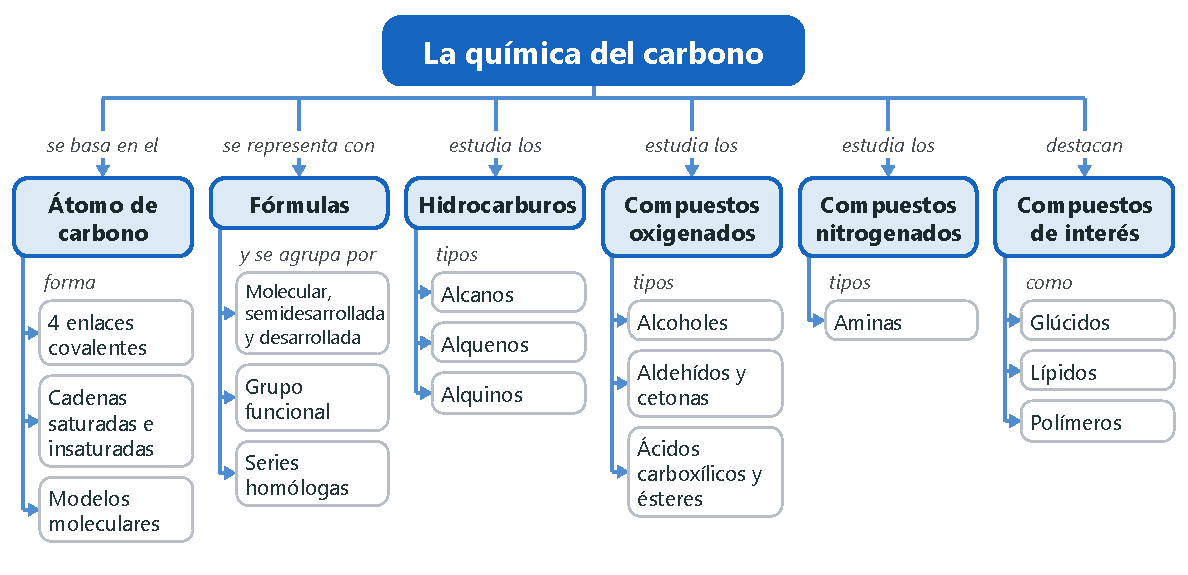
\includegraphics[width=\textwidth]{images/mapas_conceptuales/mapa_UD4}
\end{figure}

%========================================================================================
%\section*{Para empezar: la vida en la Tierra}
%\addcontentsline{toc}{section}{Para empezar: la vida en la Tierra}
%========================================================================================
%
%Las moléculas grandes se construyen con átomos que se «enganchan» con facilidad a otros átomos. El átomo de carbono, con cuatro electrones en su última capa, tiene esa cualidad: puede unirse a otros cuatro átomos, incluidos otros carbonos, y formar cadenas y anillos enormes. Por eso decimos que la vida en la Tierra está basada en el carbono.
%
%En las células hay cuatro tipos de moléculas esenciales, las \textbf{biomoléculas}:
%\begin{itemize}
%    \item Los \textbf{ácidos nucleicos} (ADN y ARN), que guardan y transmiten la información genética de generación en generación.
%    \item Las \textbf{proteínas}, formadas por cientos de moléculas más pequeñas, los \textbf{aminoácidos}. Cada aminoácido tiene un grupo amino (\ch{-NH2}) en un extremo y un grupo ácido (\ch{-COOH}) en el otro.
%    \item Los \textbf{hidratos de carbono} o \textbf{glúcidos}, que proporcionan el combustible a las células: glucosa, fructosa, sacarosa\ldots{} Muchas moléculas de glucosa enlazadas forman el almidón y la celulosa: la camiseta de algodón que llevas (celulosa) está hecha del mismo «ladrillo» que el azúcar que echas en el desayuno.
%    \item Los \textbf{lípidos}, moléculas orgánicas insolubles en agua, como las grasas y los aceites, que almacenan energía de forma muy eficiente.
%\end{itemize}
%
%Conocer la composición de la materia viva ayuda a garantizar una alimentación suficiente y sana (\textbf{ODS 2}, \emph{Hambre cero}) y a prevenir y tratar enfermedades, desarrollar vacunas y medicamentos (\textbf{ODS 3}, \emph{Salud y bienestar}). En esta unidad estudiaremos cómo es el átomo de carbono, cómo se unen los carbonos entre sí, cómo se nombran y formulan los compuestos del carbono más sencillos y qué propiedades y aplicaciones tienen.
%
%\begin{exercise}
%    ¿Por qué decimos que la vida en la Tierra está basada en el carbono?
%    \begin{solu}
%        Porque el carbono, con \textcolor{red}{cuatro electrones de valencia}, puede formar cuatro enlaces y unirse a otros átomos de carbono, dando lugar a las \textcolor{red}{cadenas y moléculas grandes} de las que están hechos los seres vivos (las biomoléculas).
%    \end{solu}
%\end{exercise}
%
%\begin{exercise}
%    ¿Qué moléculas transmiten la información genética? ¿De qué moléculas más pequeñas están formadas las proteínas y qué estructura tienen?
%    \begin{solu}
%        La información genética la transmiten los \textcolor{red}{ácidos nucleicos} (ADN y ARN). Las proteínas están formadas por \textcolor{red}{aminoácidos}, que tienen un \textcolor{red}{grupo amino}, \ch{-NH2}, y un \textcolor{red}{grupo ácido (carboxilo)}, \ch{-COOH}.
%    \end{solu}
%\end{exercise}
%
%\begin{exercise}
%    ¿Qué moléculas suministran el combustible a las células? ¿Por qué el texto compara el algodón con el azúcar?
%    \begin{solu}
%        Los \textcolor{red}{hidratos de carbono}, como la glucosa, la fructosa o la sacarosa. El algodón (celulosa) y el azúcar son \textcolor{red}{hidratos de carbono} y tienen el mismo «ladrillo» básico: la glucosa.
%    \end{solu}
%\end{exercise}
%
%\begin{exercise}
%    ¿Qué característica común tienen los lípidos y qué función cumplen? ¿Qué relación tienen las biomoléculas con los ODS 2 y 3?
%    \begin{solu}
%        Los lípidos son \textcolor{red}{insolubles en agua} y sirven para \textcolor{red}{almacenar energía}. Respuesta libre sobre los ODS: necesitamos ingerir a diario materia orgánica (glúcidos, lípidos, proteínas) para alimentarnos (ODS 2), y conocer las biomoléculas permite combatir la malnutrición y las enfermedades, y desarrollar vacunas y medicamentos (ODS 3).
%    \end{solu}
%\end{exercise}

%========================================================================================
\section{¿Qué características tiene el átomo de carbono?}
%========================================================================================

La vida en la Tierra se basa en la química del carbono, que tiene una gran facilidad para formar largas cadenas y anillos que pueden incluir otros elementos de la materia viva, como el hidrógeno, el oxígeno, el nitrógeno, el fósforo o el azufre. Se conocen más de diez millones de compuestos del carbono, muchos más que de todos los demás elementos juntos.

El carbono (\(Z = 6\)) está en el grupo 14 y el período 2 del sistema periódico. Su configuración electrónica es \conf{1s^2~2s^2~2p^2}: tiene \textbf{cuatro electrones de valencia} y le faltan otros cuatro para completar su capa de valencia. Por eso:
\begin{itemize}
    \item El carbono completa su capa uniéndose a otros átomos mediante \textbf{cuatro enlaces covalentes}, muy estables.
    \item Estos cuatro enlaces se dirigen en el espacio hacia los \textbf{vértices de un tetraedro regular}, con el átomo de carbono en el centro (figura~\ref{fig:tetraedro}).
\end{itemize}

\begin{figure}[H]
    \centering
    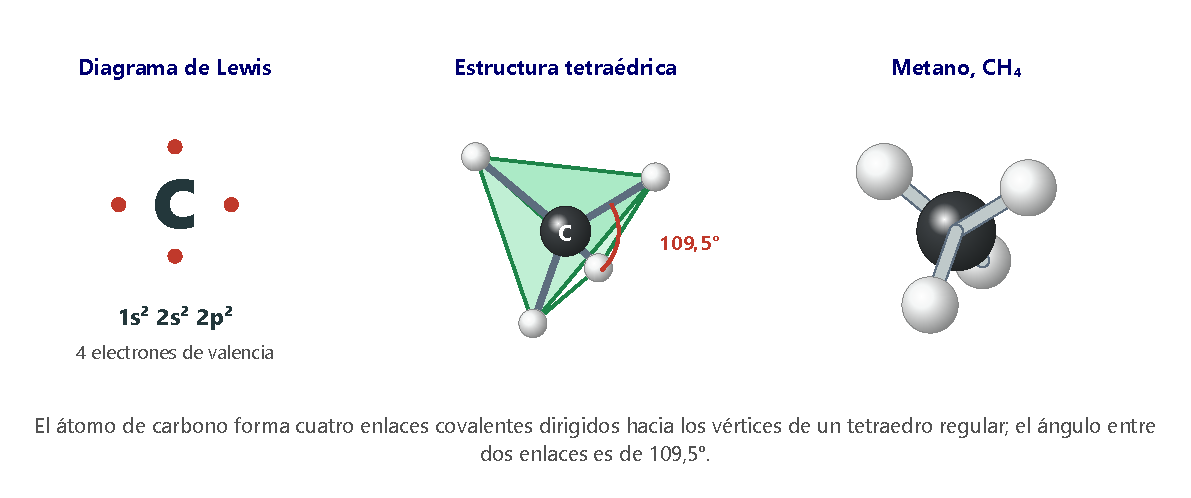
\includegraphics[width=0.95\textwidth]{images/UD4/tetraedro}
    \caption{Diagrama de Lewis y estructura tetraédrica del átomo de carbono.}
    \label{fig:tetraedro}
\end{figure}

\subsection{Los modelos moleculares en la química del carbono}

La estructura tetraédrica del carbono determina la forma de las moléculas de sus compuestos. Para ver cómo se orientan los átomos en el espacio usamos \textbf{modelos moleculares}, físicos o virtuales. Los más usados son los \textbf{modelos de bolas y varillas}: los átomos se representan con esferas y los enlaces con varillas, de modo que se aprecian los ángulos entre enlaces y si estos son simples, dobles o triples.

Por convenio, los átomos de carbono se dibujan de color gris o negro, los de hidrógeno de blanco, los de oxígeno de rojo, los de nitrógeno de azul y los de cloro o flúor de verde (figura~\ref{fig:modelos_moleculares}).

\begin{figure}[H]
    \centering
    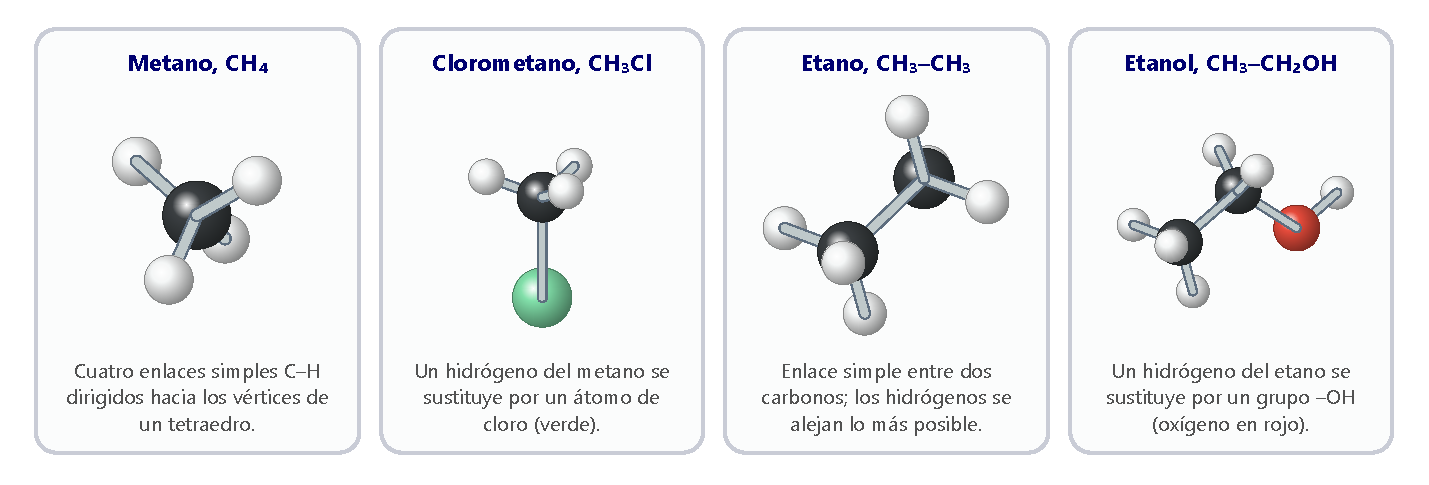
\includegraphics[width=\textwidth]{images/UD4/modelos_moleculares}
    \caption{Modelos de bolas y varillas de algunos compuestos del carbono.}
    \label{fig:modelos_moleculares}
\end{figure}

\begin{exercise}
    Observa el modelo de bolas y varillas del metano. ¿Es una molécula plana o tridimensional?
    \begin{solu}
        Es \textcolor{red}{tridimensional}: los cuatro hidrógenos están en los vértices de un tetraedro.
    \end{solu}
\end{exercise}

\subsection*{Actividades de consolidación: el átomo de carbono}

\begin{exercise}
    A comienzos del siglo \textsc{xix} se creía que los compuestos de los seres vivos solo podían formarse gracias a una «fuerza vital» que había en ellos, y por eso se llamaron \emph{compuestos orgánicos}. En 1828, Friedrich Wöhler sintetizó en su laboratorio la urea, un compuesto orgánico, sin ninguna fuerza vital. Desde entonces se habla de \emph{compuestos del carbono}.
    \begin{enumerate}[label=\alph*)]
        \item ¿Por qué hasta el siglo \textsc{xix} se distinguía entre compuestos orgánicos e inorgánicos?
        \item Según aquel criterio, clasifica: almidón, cloruro de sodio, glucosa, celulosa, agua, hemoglobina, arginina, triptófano, metano y etanol.
    \end{enumerate}
    \begin{solu}
        a) Porque se creía que los compuestos de los seres vivos solo se podían formar gracias a una \textcolor{red}{fuerza vital} presente en ellos.
        b) Orgánicos (los producen los seres vivos): \textcolor{red}{almidón, glucosa, celulosa, hemoglobina, arginina, triptófano, metano} (se forma al descomponerse la materia orgánica) y \textcolor{red}{etanol} (se forma en la fermentación). Inorgánicos: \textcolor{red}{cloruro de sodio y agua}.
    \end{solu}
\end{exercise}

\begin{exercise}
    Escribe la configuración electrónica del carbono y dibuja su diagrama de Lewis. a) ¿Cuántos electrones de valencia tiene? b) ¿Cuántos le faltan para completar el nivel 2? c) ¿Cuántos enlaces covalentes puede formar?
    \begin{solu}
        \conf{1s^2~2s^2~2p^2}; Lewis: \quad\chemfig{\charge{90=\.,0=\.,270=\.,180=\.}{C}}\quad.
        a) \textcolor{red}{Cuatro}. b) \textcolor{red}{Cuatro} (el nivel 2 se completa con ocho electrones). c) \textcolor{red}{Cuatro} enlaces covalentes.
    \end{solu}
\end{exercise}

\begin{exercise}
    En la figura~\ref{fig:modelos_moleculares}, identifica: a) dos compuestos con dos átomos de carbono; b) dos compuestos con un solo carbono; c) un compuesto con cloro; d) un compuesto con oxígeno.
    \begin{solu}
        a) El \textcolor{red}{etano} y el \textcolor{red}{etanol}. b) El \textcolor{red}{metano} y el \textcolor{red}{clorometano}. c) El \textcolor{red}{clorometano}. d) El \textcolor{red}{etanol}.
    \end{solu}
\end{exercise}

\begin{exercise}
    Sitúa el carbono en el sistema periódico: a) ¿en qué grupo y período está? b) ¿Cuál es su número atómico?
    \begin{solu}
        a) \textcolor{red}{Grupo 14, período 2}. b) \(Z = \textcolor{red}{6}\).
    \end{solu}
\end{exercise}

\begin{exercise}
    Dibuja la estructura tetraédrica del átomo de carbono. ¿Qué tipo de enlace lo une a los otros cuatro átomos?
    \begin{solu}
        El carbono ocupa el centro de un tetraedro y sus cuatro enlaces apuntan a los vértices, formando ángulos de \ang{109.5} (figura~\ref{fig:tetraedro}). Son \textcolor{red}{enlaces covalentes}.
    \end{solu}
\end{exercise}

\begin{exercise}
    Dibuja una cadena de dos átomos de carbono unidos y complétala con seis hidrógenos, uno en cada vértice libre de los tetraedros. ¿Qué compuesto es?
    \begin{solu}
        Es el \textcolor{red}{etano}, \ch{CH3-CH3}: cada carbono está unido al otro carbono y a tres hidrógenos (figura~\ref{fig:modelos_moleculares}).
    \end{solu}
\end{exercise}

%========================================================================================
\section{¿Cómo son los enlaces carbono-carbono?}
%========================================================================================

El átomo de carbono puede unirse mediante sus cuatro enlaces covalentes a átomos de otros elementos (hidrógeno, oxígeno, nitrógeno, halógenos\ldots), pero sobre todo a otros átomos de carbono, formando \textbf{cadenas carbonadas}, que son el esqueleto de los compuestos del carbono.

Dos átomos de carbono pueden unirse entre sí mediante un enlace simple, doble o triple, según compartan uno, dos o tres pares de electrones (figura~\ref{fig:enlaces_cc}):

\begin{center}
    % --- tabla antigua ---
    % \begin{tblr}{colspec={X[l]X[l]X[l]}, hlines, vlines, row{1}={bg=ocre!85, fg=white, font=\bfseries}, cells={font=\small}}
        % Enlace simple, C--C & Enlace doble, C=C & Enlace triple, C\(\equiv\)C \\
        % Comparten \textbf{un par} de electrones. & Comparten \textbf{dos pares} de electrones. & Comparten \textbf{tres pares} de electrones. \\
        % Estructura \textbf{tridimensional}. A cada carbono le quedan tres enlaces para unirse a otros átomos. & Los dos carbonos y los átomos unidos a ellos están en el \textbf{mismo plano}. A cada carbono le quedan dos enlaces. & Los dos carbonos y los átomos unidos a ellos están en \textbf{línea recta}. A cada carbono le queda un enlace. \\
        % Etano: \ch{CH3-CH3} & Eteno: \ch{CH2=CH2} & Etino: \ch{CH+CH} \\
    % \end{tblr}
    % --- tabla nueva ---
    {\small
    \begin{tabular}{@{}L{0.29\linewidth} L{0.29\linewidth} L{0.29\linewidth}@{}}
        \toprule
        \textbf{Enlace simple, C--C} & \textbf{Enlace doble, C=C} & \textbf{Enlace triple, C\(\equiv\)C} \\
        \midrule
        Comparten \textbf{un par} de electrones. & Comparten \textbf{dos pares} de electrones. & Comparten \textbf{tres pares} de electrones. \\[3pt]
        Estructura \textbf{tridimensional}. A cada carbono le quedan tres enlaces para unirse a otros átomos. & Los dos carbonos y los átomos unidos a ellos están en el \textbf{mismo plano}. A cada carbono le quedan dos enlaces. & Los dos carbonos y los átomos unidos a ellos están en \textbf{línea recta}. A cada carbono le queda un enlace. \\[3pt]
        Etano: \ch{CH3-CH3} & Eteno: \ch{CH2=CH2} & Etino: \ch{CH+CH} \\
        \bottomrule
    \end{tabular}
    }
\end{center}

\begin{figure}[H]
    \centering
    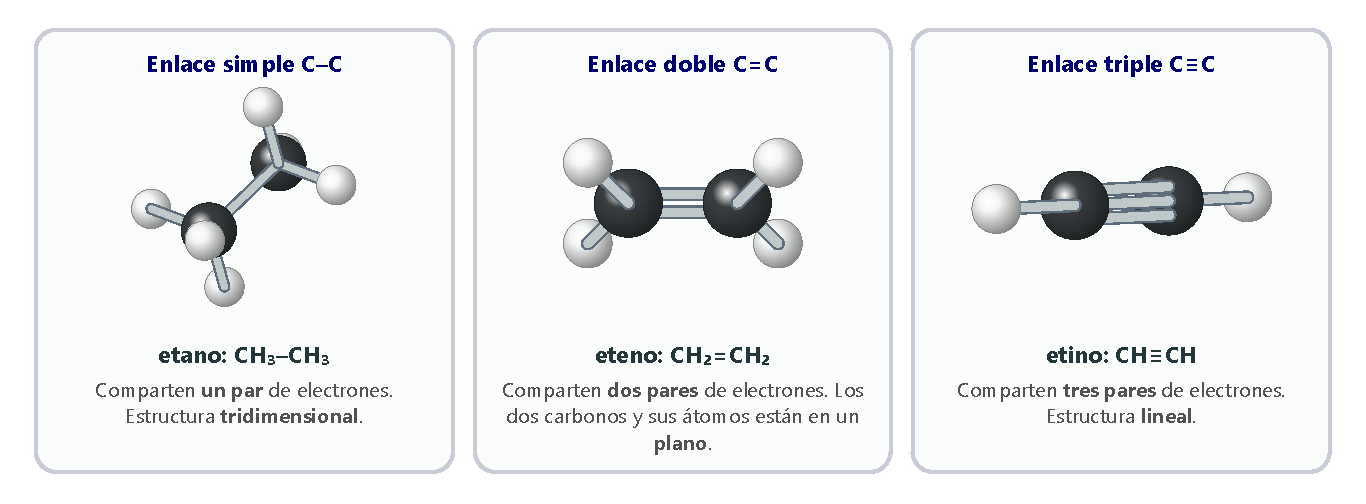
\includegraphics[width=\textwidth]{images/UD4/enlaces_cc}
    \caption{Modelos moleculares del etano, el eteno y el etino.}
    \label{fig:enlaces_cc}
\end{figure}

\subsection{¿Qué diferencia hay entre una cadena saturada y una insaturada?}

\begin{itemize}
    \item Una \textbf{cadena saturada} solo tiene enlaces carbono-carbono simples. Por ejemplo, el pentano: \ch{CH3-CH2-CH2-CH2-CH3}.
    \item Una \textbf{cadena insaturada} tiene, al menos, un enlace carbono-carbono doble o triple. Por ejemplo: \ch{CH3-CH=CH-CH2-CH3} y \ch{CH3-C+CH}.
\end{itemize}

\begin{exercise}
    ¿Cuántos electrones comparten dos átomos de carbono unidos por un doble enlace? ¿Y por un triple enlace?
    \begin{solu}
        Por un doble enlace, \textcolor{red}{cuatro} electrones (dos pares); por un triple enlace, \textcolor{red}{seis} electrones (tres pares).
    \end{solu}
\end{exercise}

\subsection*{Actividades de consolidación: los enlaces carbono-carbono}

\begin{exercise}
    Señala si es verdadero o falso y justifica tu respuesta:
    \begin{enumerate}[label=\alph*)]
        \item Si en una cadena hay dos carbonos unidos por un enlace doble o triple, la cadena no puede ser saturada.
        \item Dos carbonos que comparten dos pares de electrones están unidos por un enlace triple.
        \item Los enlaces entre los átomos de carbono son iónicos.
        \item Una molécula en la que todos los enlaces entre carbonos son simples es plana.
    \end{enumerate}
    \begin{solu}
        a) \textcolor{red}{Verdadero}: es insaturada. b) \textcolor{red}{Falso}: es un enlace doble. c) \textcolor{red}{Falso}: son covalentes. d) \textcolor{red}{Falso}: es tridimensional.
    \end{solu}
\end{exercise}

\begin{exercise}
    Escribe la fórmula de una cadena carbonada de cuatro carbonos que tenga: a) solo enlaces simples; b) al menos un doble enlace; c) al menos un triple enlace.
    \begin{solu}
        Respuesta abierta. Por ejemplo: a) \textcolor{red}{\ch{CH3-CH2-CH2-CH3}}; b) \textcolor{red}{\ch{CH2=CH-CH2-CH3}}; c) \textcolor{red}{\ch{CH+C-CH2-CH3}}.
    \end{solu}
\end{exercise}

\begin{exercise}
    Indica si cada enunciado corresponde al enlace simple, al doble o al triple:
    a) los carbonos comparten tres pares de electrones; b) se representa C=C; c) estructura tridimensional; d) se representa C--C; e) los carbonos y los átomos unidos a ellos están en un plano; f) estructura lineal; g) los carbonos comparten un par de electrones; h) los carbonos comparten dos pares de electrones.
    \begin{solu}
        Enlace simple: \textcolor{red}{c), d) y g)}. Enlace doble: \textcolor{red}{b), e) y h)}. Enlace triple: \textcolor{red}{a) y f)}.
    \end{solu}
\end{exercise}

\begin{exercise}
    En un modelo de bolas y varillas, ¿cómo distinguirías una molécula con un enlace C--C simple, otra con uno doble y otra con uno triple?
    \begin{solu}
        Por el número de varillas entre los dos carbonos (\textcolor{red}{una, dos o tres}) y por la forma: con enlace simple la molécula es \textcolor{red}{tridimensional}; con doble, los átomos unidos a los carbonos están en un \textcolor{red}{plano}; con triple, en \textcolor{red}{línea recta} (figura~\ref{fig:enlaces_cc}).
    \end{solu}
\end{exercise}

%========================================================================================
\section{¿Cómo son las fórmulas en la química del carbono?}
%========================================================================================

Una \textbf{fórmula química} es la expresión abreviada de la composición de una molécula. Para los compuestos del carbono usamos cuatro tipos de fórmulas. Por ejemplo, para el butano:

\begin{center}
    % --- tabla antigua ---
    % \begin{tblr}{colspec={Q[l,m,0.24\textwidth]X[l,m]}, hlines, vlines, column{1}={font=\bfseries\small}, cells={font=\small}}
        % Fórmula molecular & Indica cuántos átomos de cada elemento hay en la molécula, pero no cómo están unidos. Butano: \ch{C4H10}. \\
        % Fórmula semidesarrollada & Solo se escriben los enlaces entre carbonos (y con los grupos funcionales); los demás átomos se agrupan con el carbono al que están unidos. Butano: \ch{CH3-CH2-CH2-CH3}. \\
        % Fórmula desarrollada o estructural & Muestra todos los átomos y todos los enlaces, pero no su disposición en el espacio. Butano: \setchemfig{atom sep=1.7em}\chemfig{H-C(-[2]H)(-[6]H)-C(-[2]H)(-[6]H)-C(-[2]H)(-[6]H)-C(-[2]H)(-[6]H)-H} \\
        % Fórmula geométrica & Representa en el plano la molécula tridimensional: los enlaces que salen hacia el observador se dibujan con cuñas, y los que se alejan, con cuñas de trazo discontinuo. Es lo más parecido a un modelo de bolas y varillas. \\
    % \end{tblr}
    % --- tabla nueva ---
    {\small
    \begin{tabular}{@{}l L{0.78\linewidth}@{}}
        \toprule
        \textbf{Fórmula molecular} & Indica cuántos átomos de cada elemento hay en la molécula, pero no cómo están unidos. Butano: \ch{C4H10}. \\[3pt]
        \textbf{Fórmula semidesarrollada} & Solo se escriben los enlaces entre carbonos (y con los grupos funcionales); los demás átomos se agrupan con el carbono al que están unidos. Butano: \ch{CH3-CH2-CH2-CH3}. \\[3pt]
        \textbf{Fórmula desarrollada o estructural} & Muestra todos los átomos y todos los enlaces, pero no su disposición en el espacio. Butano: \setchemfig{atom sep=1.7em}\chemfig{H-C(-[2]H)(-[6]H)-C(-[2]H)(-[6]H)-C(-[2]H)(-[6]H)-C(-[2]H)(-[6]H)-H} \\[3pt]
        \textbf{Fórmula geométrica} & Representa en el plano la molécula tridimensional: los enlaces que salen hacia el observador se dibujan con cuñas, y los que se alejan, con cuñas de trazo discontinuo. Es lo más parecido a un modelo de bolas y varillas. \\
        \bottomrule
    \end{tabular}
    }
\end{center}

\begin{center}
    % --- tabla antigua ---
    % \begin{tblr}{colspec={Q[l,m]Q[c,m]Q[c,m]Q[c,m]Q[c,m]}, hlines, vlines, row{1}={bg=ocre!85, fg=white, font=\bfseries\small}, column{1}={font=\bfseries\small}, cell{1}{1}={bg=ocre!85, fg=white}, cells={font=\small}}
        % Molécula & Metano & Clorometano & Eteno & Etanal \\
        % Molecular & \ch{CH4} & \ch{CH3Cl} & \ch{C2H4} & \ch{C2H4O} \\
        % Semidesarrollada & \ch{CH4} & \ch{CH3Cl} & \ch{CH2=CH2} & \ch{CH3-CHO} \\
        % Desarrollada & \chemfig{C(-[0]H)(-[2]H)(-[4]H)(-[6]H)} & \chemfig{C(-[0]H)(-[2]H)(-[4]H)(-[6]Cl)} & \chemfig{C(-[3]H)(-[5]H)=C(-[1]H)(-[7]H)} & \chemfig{H-C(-[2]H)(-[6]H)-C(=[1]O)(-[7]H)} \\
    % \end{tblr}
    % --- tabla nueva ---
    {\small
    \begin{tabular}{@{}lcccc@{}}
        \toprule
        \textbf{Molécula} & \textbf{Metano} & \textbf{Clorometano} & \textbf{Eteno} & \textbf{Etanal} \\
        \midrule
        \textbf{Molecular} & \ch{CH4} & \ch{CH3Cl} & \ch{C2H4} & \ch{C2H4O} \\[3pt]
        \textbf{Semidesarrollada} & \ch{CH4} & \ch{CH3Cl} & \ch{CH2=CH2} & \ch{CH3-CHO} \\[3pt]
        \textbf{Desarrollada} & \chemfig{C(-[0]H)(-[2]H)(-[4]H)(-[6]H)} & \chemfig{C(-[0]H)(-[2]H)(-[4]H)(-[6]Cl)} & \chemfig{C(-[3]H)(-[5]H)=C(-[1]H)(-[7]H)} & \chemfig{H-C(-[2]H)(-[6]H)-C(=[1]O)(-[7]H)} \\
        \bottomrule
    \end{tabular}
    }
\end{center}

\subsection{¿Por qué ciertos compuestos del carbono tienen propiedades parecidas? Grupo funcional y serie homóloga}

\begin{definition}[Grupo funcional]
    Un \textbf{grupo funcional} es un átomo o conjunto de átomos responsable del comportamiento químico de la molécula. Por ejemplo, todos los alcoholes tienen el grupo \ch{-OH}, que les da propiedades parecidas.
\end{definition}

\begin{definition}[Serie homóloga]
    Una \textbf{serie homóloga} es un grupo de compuestos que tienen el mismo grupo funcional pero cadenas con distinto número de átomos de carbono. Sus propiedades físicas y químicas son semejantes.
\end{definition}

En las fórmulas generales, la letra \textbf{R} (o R\('\), R\(''\)) representa un \textbf{radical}: una cadena de carbonos a la que le falta un hidrógeno, que se ha sustituido por el grupo funcional. Por ejemplo, el eteno, el propeno y el but-1-eno (con el grupo C=C) son gases en condiciones normales y reaccionan con el agua para dar alcoholes.

\subsection{¿Cómo se nombran y formulan los compuestos del carbono?}

Para formular y nombrar los compuestos del carbono se siguen las reglas de la IUPAC:
\begin{enumerate}[label=\numberballblue]
    \item Se localiza la \textbf{cadena principal}: la cadena carbonada más larga (si hay grupo funcional, la más larga que lo contenga).
    \item Se \textbf{numeran} sus carbonos empezando por el extremo más próximo al grupo funcional o, si no lo hay, a un sustituyente, de modo que los números (\emph{localizadores}) sean lo más bajos posible.
    \item Se nombran los \textbf{sustituyentes} (radicales) delante del nombre de la cadena, cada uno precedido de su localizador y un guion. Si hay varios, se separan los números con comas y se ordenan alfabéticamente.
    \item Los dobles y triples enlaces y los grupos funcionales se localizan igual, con el número delante de la terminación del nombre.
    \item El nombre tiene un \textbf{prefijo}, que indica el número de carbonos de la cadena principal, y un \textbf{sufijo}, que indica el grupo funcional.
\end{enumerate}

\begin{center}
    % --- tabla antigua ---
    % \begin{tblr}{colspec={cccccccccc}, hlines, vlines, row{1}={bg=ocre!85, fg=white, font=\bfseries}, cells={font=\small}}
        % 1 & 2 & 3 & 4 & 5 & 6 & 7 & 8 & 9 & 10 \\
        % met- & et- & prop- & but- & pent- & hex- & hept- & oct- & non- & dec- \\
    % \end{tblr}
    % --- tabla nueva ---
    {\small
    \begin{tabular}{@{}cccccccccc@{}}
        \toprule
        \textbf{1} & \textbf{2} & \textbf{3} & \textbf{4} & \textbf{5} & \textbf{6} & \textbf{7} & \textbf{8} & \textbf{9} & \textbf{10} \\
        \midrule
        met- & et- & prop- & but- & pent- & hex- & hept- & oct- & non- & dec- \\
        \bottomrule
    \end{tabular}
    }
\end{center}

\begin{center}
    % --- tabla antigua ---
    % \begin{tblr}{colspec={lcccl}, hlines, vlines, row{1}={bg=ocre!85, fg=white, font=\bfseries}, cells={font=\small}}
        % Serie homóloga & Grupo funcional & Sufijo & Ejemplo & Nombre \\
        % Alcanos & C--C & -ano & \ch{CH3-CH3} & etano \\
        % Alquenos & C=C & -eno & \ch{CH2=CH2} & eteno \\
        % Alquinos & C\(\equiv\)C & -ino & \ch{CH+CH} & etino \\
        % Alcoholes & \ch{-OH} (hidroxilo) & -ol & \ch{CH3OH} & metanol \\
        % Aldehídos & \ch{-CHO} (carbonilo) & -al & \ch{H-CHO} & metanal \\
        % Cetonas & \ch{-CO\bond{single}} (carbonilo) & -ona & \ch{CH3-CO-CH3} & propanona \\
        % Ácidos carboxílicos & \ch{-COOH} (carboxilo) & -oico & \ch{CH3-COOH} & ácido etanoico \\
        % Ésteres & \ch{-COO\bond{single}} & -oato de -ilo & \ch{CH3-COO-CH3} & etanoato de metilo \\
        % Aminas & \ch{-NH2} (amino) & -amina & \ch{CH3-CH2-NH2} & etilamina \\
    % \end{tblr}
    % --- tabla nueva ---
    {\small
    \begin{tabular}{@{}lcccl@{}}
        \toprule
        \textbf{Serie homóloga} & \textbf{Grupo funcional} & \textbf{Sufijo} & \textbf{Ejemplo} & \textbf{Nombre} \\
        \midrule
        Alcanos & C--C & -ano & \ch{CH3-CH3} & etano \\[3pt]
        Alquenos & C=C & -eno & \ch{CH2=CH2} & eteno \\[3pt]
        Alquinos & C\(\equiv\)C & -ino & \ch{CH+CH} & etino \\[3pt]
        Alcoholes & \ch{-OH} (hidroxilo) & -ol & \ch{CH3OH} & metanol \\[3pt]
        Aldehídos & \ch{-CHO} (carbonilo) & -al & \ch{H-CHO} & metanal \\[3pt]
        Cetonas & \ch{-CO\bond{single}} (carbonilo) & -ona & \ch{CH3-CO-CH3} & propanona \\[3pt]
        Ácidos carboxílicos & \ch{-COOH} (carboxilo) & -oico & \ch{CH3-COOH} & ácido etanoico \\[3pt]
        Ésteres & \ch{-COO\bond{single}} & -oato de -ilo & \ch{CH3-COO-CH3} & etanoato de metilo \\[3pt]
        Aminas & \ch{-NH2} (amino) & -amina & \ch{CH3-CH2-NH2} & etilamina \\
        \bottomrule
    \end{tabular}
    }
\end{center}

Por ejemplo, el compuesto
\[ \chemfig{CH_3-C(-[6]CH_3)=CH-CH_2-CH_3} \]
tiene una cadena principal de cinco carbonos con un doble enlace entre los carbonos 2 y 3 y un radical metilo en el carbono 2: es el \textbf{2-metilpent-2-eno}.

\begin{example}
    Nombra estos compuestos:
    \[ \text{a)}\ \ch{CH2OH-CH2-CH2-CH3} \qquad \text{b)}\ \ch{CH3-CH2-CH2-CO-CH3} \]

    a) Tiene cuatro carbonos (prefijo \emph{but-}) y un grupo \ch{-OH} en el carbono 1 (sufijo \emph{-ol}): \textcolor{red}{butan-1-ol}.

    b) Tiene cinco carbonos (prefijo \emph{pent-}) y un grupo \ch{C=O} en el interior de la cadena, en el carbono 2 numerando desde la derecha (sufijo \emph{-ona}): \textcolor{red}{pentan-2-ona}.
\end{example}

\begin{exercise}
    La fórmula semidesarrollada del propano es \ch{CH3-CH2-CH3}. Escribe su fórmula molecular y su fórmula desarrollada.
    \begin{solu}
        Molecular: \textcolor{red}{\ch{C3H8}}. Desarrollada: \chemfig{H-C(-[2]H)(-[6]H)-C(-[2]H)(-[6]H)-C(-[2]H)(-[6]H)-H}.
    \end{solu}
\end{exercise}

\begin{exercise}
    Escribe las fórmulas molecular y desarrollada del etano, \ch{CH3-CH3}, y del pentano, \ch{CH3-CH2-CH2-CH2-CH3}.
    \begin{solu}
        \textcolor{red}{Etano}, \ch{C2H6}:
        \[ \chemfig{H-C(-[2]H)(-[6]H)-C(-[2]H)(-[6]H)-H} \]
        \textcolor{red}{Pentano}, \ch{C5H12}:
        \[ \chemfig{H-C(-[2]H)(-[6]H)-C(-[2]H)(-[6]H)-C(-[2]H)(-[6]H)-C(-[2]H)(-[6]H)-C(-[2]H)(-[6]H)-H} \]
    \end{solu}
\end{exercise}

\begin{exercise}
    Explica la diferencia entre grupo funcional y serie homóloga.
    \begin{solu}
        Un \textcolor{red}{grupo funcional} es el átomo o grupo de átomos responsable del comportamiento químico de una molécula. Una \textcolor{red}{serie homóloga} es el conjunto de compuestos que tienen el mismo grupo funcional y se diferencian en el número de carbonos de la cadena.
    \end{solu}
\end{exercise}

\begin{exercise}
    Observa estos compuestos: A: \ch{CH3-CH2-CH2-CH3}; B: \ch{CH2=CH-CH2-CH3}; C: \ch{CH2=CH-CH2-CH2-CH3}; D: \ch{CH3-CH2-CH2-CH2OH}; E: \ch{CH3-CO-CH2-CH3}.
    \begin{enumerate}[label=\alph*)]
        \item Identifica el grupo funcional y la serie homóloga de cada uno.
        \item ¿Cuáles tienen grupos oxigenados?
        \item ¿Cuáles pertenecen a la misma serie homóloga?
    \end{enumerate}
    \begin{solu}
        a) A: C--C, \textcolor{red}{alcano}; B y C: C=C, \textcolor{red}{alquenos}; D: \ch{-OH}, \textcolor{red}{alcohol}; E: C=O, \textcolor{red}{cetona}.
        b) \textcolor{red}{D y E}. c) \textcolor{red}{B y C} (but-1-eno y pent-1-eno).
    \end{solu}
\end{exercise}

\begin{exercise}
    ¿Qué diferencia hay entre el grupo funcional de un aldehído y el de una cetona? ¿Qué elemento distinto del carbono y el hidrógeno tiene el grupo funcional de una amina?
    \begin{solu}
        Los dos tienen el grupo carbonilo, C=O, pero en los \textcolor{red}{aldehídos está en un extremo} de la cadena (\ch{-CHO}) y en las \textcolor{red}{cetonas, en el interior} (\ch{-CO\bond{single}}). El grupo amino de las aminas tiene \textcolor{red}{nitrógeno}.
    \end{solu}
\end{exercise}

\begin{exercise}
    Indica el grupo funcional de estos compuestos, numera sus carbonos y nómbralos: a) \ch{CH3-CH=CH-CH3}; b) \ch{CH3-CH2-CH2-COOH}; c) \ch{CH3-CH2-CHO}.
    \begin{solu}
        a) C=C; da igual el extremo por el que se empiece: \textcolor{red}{but-2-eno}.
        b) \ch{-COOH}; el carbono 1 es el del grupo carboxilo: \textcolor{red}{ácido butanoico}.
        c) \ch{-CHO}; el carbono 1 es el del grupo aldehído: \textcolor{red}{propanal}.
    \end{solu}
\end{exercise}

\begin{exercise}
    Formula estos compuestos: a) 4-metilhex-2-eno; b) 4-metilhex-3-eno; c) but-2-ino; d) pentan-2-ol.
    \begin{solu}
        \[ \text{a)}\ \textcolor{red}{\chemfig{CH_3-CH=CH-CH(-[6]CH_3)-CH_2-CH_3}} \]

        \[ \text{b)}\ \textcolor{red}{\chemfig{CH_3-CH_2-CH=C(-[6]CH_3)-CH_2-CH_3}} \]

        c) \textcolor{red}{\ch{CH3-C+C-CH3}} \qquad d) \textcolor{red}{\ch{CH3-CHOH-CH2-CH2-CH3}}
    \end{solu}
\end{exercise}

\begin{exercise}
    Un alumno ha nombrado este compuesto como 2-etilbutano:
    \[ \chemfig{CH_3-CH(-[6]CH_2-[0]CH_3)-CH_2-CH_3} \]
    ¿Es correcto? ¿Cuál es la cadena más larga? Nómbralo bien.
    \begin{solu}
        \textcolor{red}{No}: la cadena más larga no es la horizontal de cuatro carbonos, sino la que sigue por el radical etilo, que tiene \textcolor{red}{cinco carbonos}. El compuesto tiene un metilo en el carbono 3: es el \textcolor{red}{3-metilpentano}.
    \end{solu}
\end{exercise}

\subsection*{Actividades de consolidación: las fórmulas de los compuestos del carbono}

\begin{exercise}
    Identifica el grupo funcional de estas moléculas, numera sus carbonos y nómbralas: a) \ch{CH2=CH-CH3}; b) \ch{CH3-CH2-CH3}; c) \ch{CH3-CH2-CH2OH}; d) \ch{CH3-CO-CH3}; e) \ch{CH+C-CH3}; f) \ch{CH3-CH2-COOH}; g) \ch{CH3-CHO}; h) \ch{CH3-CHOH-CH3}.
    \begin{solu}
        a) Alqueno, \textcolor{red}{propeno}. b) Alcano, \textcolor{red}{propano}. c) Alcohol, \textcolor{red}{propan-1-ol}. d) Cetona, \textcolor{red}{propanona}. e) Alquino, \textcolor{red}{propino}. f) Ácido carboxílico, \textcolor{red}{ácido propanoico}. g) Aldehído, \textcolor{red}{etanal}. h) Alcohol, \textcolor{red}{propan-2-ol}.
    \end{solu}
\end{exercise}

\begin{exercise}
    Indica la serie homóloga y el grupo funcional de: a) \ch{CH3-CHO}; b) \ch{CH3-COOH}.
    \begin{solu}
        a) \textcolor{red}{Aldehído}, grupo carbonilo terminal, \ch{-CHO}. b) \textcolor{red}{Ácido carboxílico}, grupo carboxilo, \ch{-COOH}.
    \end{solu}
\end{exercise}

\begin{exercise}
    Localiza la cadena principal, numérala correctamente y nombra estos compuestos:
    \[ \text{a)}\ \chemfig{CH_3-CH_2-CH(-[6]CH_3)-CH_2-CH_2-CH_3} \]
    \[ \text{b)}\ \chemfig{CH_3-CH_2-CH(-[6]CH_3)-C~C-CHO} \]
    \begin{solu}
        a) Cadena de seis carbonos; se numera desde la izquierda para que el metilo tenga el localizador más bajo (3 en vez de 4): \textcolor{red}{3-metilhexano}.
        b) El grupo aldehído manda: el carbono 1 es el del \ch{-CHO}. Cadena de seis carbonos con un triple enlace en el carbono 2 y un metilo en el 4: \textcolor{red}{4-metilhex-2-inal}.
    \end{solu}
\end{exercise}

%========================================================================================
\section{¿Qué propiedades presentan los compuestos del carbono?}
%========================================================================================

La mayoría de los compuestos del carbono comparten estas características:
\begin{itemize}
    \item Están formados por \textbf{muy pocos elementos}: sobre todo C, H, O y N, y a veces Cl, Br, I, S o P. Por ejemplo: \ch{CH3-CHO}, \ch{CH+CH}, \ch{CH3-CH2-CH2OH}, \ch{CH3-CH2-NH-CH3}, \ch{CH3Cl}.
    \item Sus reacciones químicas suelen ser \textbf{muy lentas}. Sin embargo, \textbf{arden} en presencia de oxígeno (reacción de \textbf{combustión}) y producen dióxido de carbono y agua, desprendiendo mucha energía. Por eso muchos se usan como combustibles. Por ejemplo, en un mechero Bunsen se quema propano:
    \[ \ch{C3H8 (g) + 5 O2 (g) -> 3 CO2 (g) + 4 H2O (g)} \]
    \item Muchos son \textbf{poco estables frente al calor} y se descomponen al calentarlos. Por ejemplo, al calentar una disolución de urea:
    \[ \ch{CON2H4 + H2O ->[calor] CO2 + 2 NH3} \]
\end{itemize}

\subsection{La solubilidad de los compuestos del carbono}

Para saber si un compuesto del carbono se disuelve en agua (disolvente polar) o en disolventes apolares (gasolina, benceno, tetracloruro de carbono\ldots), hay que fijarse en los \textbf{grupos polares} (\ch{-OH}, \ch{-COOH}, \ch{-NH2}\ldots) y en la parte apolar (la cadena de carbonos e hidrógenos) de sus moléculas:

\begin{center}
    % --- tabla antigua ---
    % \begin{tblr}{colspec={X[l]X[l]X[l]X[l]}, hlines, vlines, row{1}={bg=ocre!85, fg=white, font=\bfseries\small}, cells={font=\small}}
        % Varios grupos polares & Molécula pequeña con un grupo polar & Molécula muy grande con un grupo polar & Sin grupos polares \\
        % \textbf{Muy solubles en agua}. Ejemplo: los azúcares (glucosa, sacarosa) y la glicerina, con muchos grupos \ch{-OH}. & \textbf{Solubles en agua} (por su grupo polar) \textbf{y en disolventes apolares} (por su parte apolar). Ejemplo: el etanol, \ch{CH3-CH2OH}. & \textbf{Insolubles en agua} y solubles en disolventes apolares. Ejemplo: el ácido oleico de los aceites, con una cadena de 17 carbonos. & \textbf{Insolubles en agua} y solubles en disolventes apolares. Ejemplo: los hidrocarburos, como el benceno, \ch{C6H6}, o la gasolina. \\
    % \end{tblr}
    % --- tabla nueva ---
    {\small
    \begin{tabular}{@{}L{0.21\linewidth} L{0.21\linewidth} L{0.21\linewidth} L{0.21\linewidth}@{}}
        \toprule
        \textbf{Varios grupos polares} & \textbf{Molécula pequeña con un grupo polar} & \textbf{Molécula muy grande con un grupo polar} & \textbf{Sin grupos polares} \\
        \midrule
        \textbf{Muy solubles en agua}. Ejemplo: los azúcares (glucosa, sacarosa) y la glicerina, con muchos grupos \ch{-OH}. & \textbf{Solubles en agua} (por su grupo polar) \textbf{y en disolventes apolares} (por su parte apolar). Ejemplo: el etanol, \ch{CH3-CH2OH}. & \textbf{Insolubles en agua} y solubles en disolventes apolares. Ejemplo: el ácido oleico de los aceites, con una cadena de 17 carbonos. & \textbf{Insolubles en agua} y solubles en disolventes apolares. Ejemplo: los hidrocarburos, como el benceno, \ch{C6H6}, o la gasolina. \\
        \bottomrule
    \end{tabular}
    }
\end{center}

\subsection*{Actividades de consolidación: propiedades de los compuestos del carbono}

\begin{exercise}
    ¿Cuáles de estas características son frecuentes en los compuestos del carbono? a) Tienen aspecto metálico y conducen la corriente. b) Están formados por muy pocos elementos. c) No se descomponen al calentarlos. d) Arden en oxígeno desprendiendo \ch{CO2} y agua.
    \begin{solu}
        Son frecuentes \textcolor{red}{b) y d)}.
    \end{solu}
\end{exercise}

\begin{exercise}
    Explica por qué el azúcar se disuelve en agua, mientras que las grasas no se disuelven en agua pero sí en disolventes como el tolueno.
    \begin{solu}
        El azúcar tiene en su molécula \textcolor{red}{muchos grupos polares} (\ch{-OH}) que interaccionan con el agua. Las grasas son moléculas \textcolor{red}{muy grandes y casi completamente apolares}: no se disuelven en agua, pero sí en disolventes apolares como el tolueno.
    \end{solu}
\end{exercise}

\begin{exercise}
    Clasifica en solubles o insolubles en agua: azúcar, glicerina, etanol, ácido acético, celulosa, ácido oleico, caucho natural, queratina y almidón.
    \begin{solu}
        Solubles: \textcolor{red}{azúcar, glicerina, etanol y ácido acético}. Insolubles: \textcolor{red}{celulosa, ácido oleico, caucho natural, queratina y almidón} (el almidón solo se dispersa en agua caliente).
    \end{solu}
\end{exercise}

\begin{exercise}
    Señala si es verdadero o falso y justifica tu respuesta:
    \begin{enumerate}[label=\alph*)]
        \item Los compuestos del carbono con uno o varios grupos polares son insolubles en agua.
        \item Las reacciones de los compuestos del carbono suelen ser muy lentas.
        \item En la combustión de los compuestos del carbono se desprende mucha energía.
        \item Los compuestos del carbono sin grupos polares son solubles en agua.
        \item Las grasas se disuelven bien en disolventes apolares, como el benceno.
    \end{enumerate}
    \begin{solu}
        a) \textcolor{red}{Falso}: los grupos polares favorecen la solubilidad en agua (si la molécula no es muy grande). b) \textcolor{red}{Verdadero}. c) \textcolor{red}{Verdadero}. d) \textcolor{red}{Falso}: son insolubles en agua. e) \textcolor{red}{Verdadero}.
    \end{solu}
\end{exercise}

%========================================================================================
\section{¿Qué son y cómo se clasifican los hidrocarburos?}
%========================================================================================

Los \textbf{hidrocarburos} son los compuestos del carbono formados \textbf{solo por carbono e hidrógeno}.

\begin{center}
    % --- tabla antigua ---
    % \begin{tblr}{colspec={X[l]X[l]X[l]}, hlines, vlines, row{1}={bg=ocre!85, fg=white, font=\bfseries}, cells={font=\small}}
        % Alcanos & Alquenos & Alquinos \\
        % Los carbonos están unidos solo por \textbf{enlaces simples}. & Hay al menos un \textbf{doble enlace} entre dos carbonos. & Hay al menos un \textbf{triple enlace} entre dos carbonos. \\
        % Cadena \textbf{saturada}. & Cadena \textbf{insaturada}. & Cadena \textbf{insaturada}. \\
        % Fórmula general: \ch{C_{n}H_{2n+2}}. & Con un doble enlace: \ch{C_{n}H_{2n}}. & Con un triple enlace: \ch{C_{n}H_{2n-2}}. \\
    % \end{tblr}
    % --- tabla nueva ---
    {\small
    \begin{tabular}{@{}L{0.29\linewidth} L{0.29\linewidth} L{0.29\linewidth}@{}}
        \toprule
        \textbf{Alcanos} & \textbf{Alquenos} & \textbf{Alquinos} \\
        \midrule
        Los carbonos están unidos solo por \textbf{enlaces simples}. & Hay al menos un \textbf{doble enlace} entre dos carbonos. & Hay al menos un \textbf{triple enlace} entre dos carbonos. \\[3pt]
        Cadena \textbf{saturada}. & Cadena \textbf{insaturada}. & Cadena \textbf{insaturada}. \\[3pt]
        Fórmula general: \ch{C_{n}H_{2n+2}}. & Con un doble enlace: \ch{C_{n}H_{2n}}. & Con un triple enlace: \ch{C_{n}H_{2n-2}}. \\
        \bottomrule
    \end{tabular}
    }
\end{center}

Todos los hidrocarburos son sustancias covalentes moleculares y apolares: son \textbf{insolubles en agua} y solubles en disolventes apolares, y son \textbf{menos densos que el agua}. Los de masa molecular pequeña son gases; a medida que la cadena es más larga, aumentan la masa molecular y las fuerzas intermoleculares, y por tanto los puntos de fusión y de ebullición.

\subsection{Los alcanos}

Los alcanos se nombran con el prefijo que indica el número de carbonos y la terminación \textbf{-ano}. Cuando un alcano pierde un hidrógeno, se obtiene un \textbf{radical alquilo}, que se nombra cambiando la terminación -ano por \textbf{-ilo} (o \textbf{-il} cuando forma parte del nombre de un compuesto):

\begin{center}
    % --- tabla antigua ---
    % \begin{tblr}{colspec={ll}, hlines, vlines, row{1}={bg=ocre!85, fg=white, font=\bfseries}, cells={font=\small}}
        % Radical & Nombre \\
        % \ch{CH3\bond{single}} & metil(o) \\
        % \ch{CH3-CH2\bond{single}} & etil(o) \\
        % \ch{CH3-CH2-CH2\bond{single}} & propil(o) \\
        % \ch{CH3-CH2-CH2-CH2\bond{single}} & butil(o) \\
    % \end{tblr}
    % --- tabla nueva ---
    {\small
    \begin{tabular}{@{}ll@{}}
        \toprule
        \textbf{Radical} & \textbf{Nombre} \\
        \midrule
        \ch{CH3\bond{single}} & metil(o) \\[3pt]
        \ch{CH3-CH2\bond{single}} & etil(o) \\[3pt]
        \ch{CH3-CH2-CH2\bond{single}} & propil(o) \\[3pt]
        \ch{CH3-CH2-CH2-CH2\bond{single}} & butil(o) \\
        \bottomrule
    \end{tabular}
    }
    \\[2ex]
    % --- tabla antigua ---
    % \begin{tblr}{colspec={ll}, hlines, vlines, row{1}={bg=ocre!85, fg=white, font=\bfseries}, cells={font=\small}}
        % Fórmula & Nombre \\
        % \ch{CH3-CH2-CH2-CH3} & butano (cadena lineal) \\
        % \chemfig{CH_3-CH(-[6]CH_3)-CH_2-CH_3} & 2-metilbutano (ramificada) \\
    % \end{tblr}
    % --- tabla nueva ---
    {\small
    \begin{tabular}{@{}ll@{}}
        \toprule
        \textbf{Fórmula} & \textbf{Nombre} \\
        \midrule
        \ch{CH3-CH2-CH2-CH3} & butano (cadena lineal) \\[3pt]
        \chemfig{CH_3-CH(-[6]CH_3)-CH_2-CH_3} & 2-metilbutano (ramificada) \\
        \bottomrule
    \end{tabular}
    }
\end{center}

Los cuatro primeros alcanos (metano, etano, propano y butano) son gases a temperatura ambiente; del pentano al heptadecano (17 carbonos) son líquidos, y a partir de ahí, sólidos (como las parafinas de las velas). El metano es el componente principal del gas natural, y el propano y el butano se venden en bombonas como combustibles domésticos.

\subsection{Los alquenos}

Los alquenos se nombran numerando la cadena desde el extremo más próximo al doble enlace. La posición del doble enlace se indica con el número del primer carbono que lo lleva, delante de la terminación \textbf{-eno}. Si hay ramificaciones, la cadena principal es la más larga que contiene el doble enlace; si hay dos o tres dobles enlaces, se usan las terminaciones \textbf{-dieno}, \textbf{-trieno}\ldots{} Por ejemplo, \ch{CH3-CH2-CH=CH-CH=CH-CH3} es el \textbf{hepta-2,4-dieno}.

\begin{center}
    % --- tabla antigua ---
    % \begin{tblr}{colspec={lcl}, hlines, vlines, row{1}={bg=ocre!85, fg=white, font=\bfseries}, cells={font=\small}}
        % Semidesarrollada & Molecular & Nombre \\
        % \ch{CH2=CH2} & \ch{C2H4} & eteno (etileno) \\
        % \ch{CH2=CH-CH3} & \ch{C3H6} & propeno \\
        % \ch{CH2=CH-CH2-CH3} & \ch{C4H8} & but-1-eno \\
        % \ch{CH3-CH=CH-CH3} & \ch{C4H8} & but-2-eno \\
    % \end{tblr}
    % --- tabla nueva ---
    {\small
    \begin{tabular}{@{}lcl@{}}
        \toprule
        \textbf{Semidesarrollada} & \textbf{Molecular} & \textbf{Nombre} \\
        \midrule
        \ch{CH2=CH2} & \ch{C2H4} & eteno (etileno) \\[3pt]
        \ch{CH2=CH-CH3} & \ch{C3H6} & propeno \\[3pt]
        \ch{CH2=CH-CH2-CH3} & \ch{C4H8} & but-1-eno \\[3pt]
        \ch{CH3-CH=CH-CH3} & \ch{C4H8} & but-2-eno \\
        \bottomrule
    \end{tabular}
    }
\end{center}

El alqueno más sencillo, el \textbf{eteno} o \textbf{etileno}, se usa para fabricar plásticos como el polietileno, el cloruro de polivinilo (PVC) o el acetato de polivinilo (PVA). También es una hormona vegetal que acelera la maduración de la fruta.

\subsection{Los alquinos}

Se nombran igual que los alquenos, pero con la terminación \textbf{-ino}:

\begin{center}
    % --- tabla antigua ---
    % \begin{tblr}{colspec={lcl}, hlines, vlines, row{1}={bg=ocre!85, fg=white, font=\bfseries}, cells={font=\small}}
        % Semidesarrollada & Molecular & Nombre \\
        % \ch{CH+CH} & \ch{C2H2} & etino (acetileno) \\
        % \ch{CH+C-CH3} & \ch{C3H4} & propino \\
        % \ch{CH+C-CH2-CH3} & \ch{C4H6} & but-1-ino \\
    % \end{tblr}
    % --- tabla nueva ---
    {\small
    \begin{tabular}{@{}lcl@{}}
        \toprule
        \textbf{Semidesarrollada} & \textbf{Molecular} & \textbf{Nombre} \\
        \midrule
        \ch{CH+CH} & \ch{C2H2} & etino (acetileno) \\[3pt]
        \ch{CH+C-CH3} & \ch{C3H4} & propino \\[3pt]
        \ch{CH+C-CH2-CH3} & \ch{C4H6} & but-1-ino \\
        \bottomrule
    \end{tabular}
    }
\end{center}

El alquino más sencillo, el \textbf{etino} o \textbf{acetileno}, es un gas incoloro que arde con una llama muy luminosa. Se usa en el soplete oxiacetilénico, cuya llama alcanza unos \qty{3500}{\degreeCelsius}, para soldar y cortar metales.

\begin{example}
    Calcula la masa molecular del propano, \ch{C3H8}, y el porcentaje de carbono que contiene.

    \(M = 3 \cdot 12 + 8 \cdot 1 = \textcolor{red}{44}\); \quad \(\% \text{C} = \dfrac{36}{44} \cdot 100 = \textcolor{red}{\qty{81.8}{\percent}}\).
\end{example}

\begin{exercise}
    Busca información sobre las aplicaciones industriales y domésticas del metano, el propano y el butano.
    \begin{solu}
        Respuesta libre. Los tres son \textcolor{red}{combustibles}: el metano (gas natural) se usa en calefacciones, cocinas y centrales térmicas, y en la industria química para fabricar hidrógeno y otros productos; el propano y el butano (gases licuados del petróleo) se venden en bombonas para cocinas, estufas, calentadores o como combustible de vehículos.
    \end{solu}
\end{exercise}

\begin{exercise}
    Tenemos dos muestras: una es pentano y la otra butano, pero no sabemos cuál es cuál. Sus puntos de ebullición son \qty{0.5}{\degreeCelsius} y \qty{36}{\degreeCelsius}. ¿A qué alcano corresponde cada uno?
    \begin{solu}
        El punto de ebullición aumenta con la longitud de la cadena: \textcolor{red}{\qty{0.5}{\degreeCelsius} corresponde al butano} (4 carbonos) y \textcolor{red}{\qty{36}{\degreeCelsius}, al pentano} (5 carbonos).
    \end{solu}
\end{exercise}

\begin{exercise}
    Formula: a) hex-2-eno; b) hex-1-eno; c) pent-2-ino; d) pent-1-ino.
    \begin{solu}
        a) \textcolor{red}{\ch{CH3-CH=CH-CH2-CH2-CH3}}; b) \textcolor{red}{\ch{CH2=CH-CH2-CH2-CH2-CH3}};
        c) \textcolor{red}{\ch{CH3-C+C-CH2-CH3}}; d) \textcolor{red}{\ch{CH+C-CH2-CH2-CH3}}.
    \end{solu}
\end{exercise}

\subsection*{Actividades de consolidación: los hidrocarburos}

\begin{exercise}
    Dibuja (o construye con modelos) las moléculas del metano, el etano, el propano y el butano teniendo en cuenta su estructura tridimensional. ¿Son estrictamente lineales sus cadenas?
    \begin{solu}
        \textcolor{red}{No}: como los enlaces de cada carbono forman ángulos de \ang{109.5}, las cadenas tienen forma de \textcolor{red}{zigzag} en el espacio (figura~\ref{fig:modelos_moleculares}).
    \end{solu}
\end{exercise}

\begin{exercise}
    Formula: a) 2-metilbuta-1,3-dieno (isopreno); b) pent-2-eno; c) 2-metilhex-3-eno.
    \begin{solu}
        \[ \text{a)}\ \textcolor{red}{\chemfig{CH_2=C(-[6]CH_3)-CH=CH_2}} \]
        \[ \text{b)}\ \textcolor{red}{\ch{CH3-CH=CH-CH2-CH3}} \]

        \[ \text{c)}\ \textcolor{red}{\chemfig{CH_3-CH(-[6]CH_3)-CH=CH-CH_2-CH_3}} \]
    \end{solu}
\end{exercise}

\begin{exercise}
    Formula: a) but-1-ino; b) but-2-ino; c) hexano; d) 3,4-dimetilhexano; e) 2-metilpentano; f) 3-metilbut-1-ino.
    \begin{solu}
        a) \textcolor{red}{\ch{CH+C-CH2-CH3}}; b) \textcolor{red}{\ch{CH3-C+C-CH3}};
        c) \textcolor{red}{\ch{CH3-CH2-CH2-CH2-CH2-CH3}};

        \[ \text{d)}\ \textcolor{red}{\chemfig{CH_3-CH_2-CH(-[6]CH_3)-CH(-[6]CH_3)-CH_2-CH_3}} \]
        \[ \text{e)}\ \textcolor{red}{\chemfig{CH_3-CH(-[6]CH_3)-CH_2-CH_2-CH_3}} \]

        \[ \text{f)}\ \textcolor{red}{\chemfig{CH~C-CH(-[6]CH_3)-CH_3}} \]
    \end{solu}
\end{exercise}

\begin{exercise}
    Nombra: a) \ch{CH3-CH=CH-CH3}; b) \ch{CH3-CH=CH2}; c) \ch{CH3-C+CH}; d) \ch{CH3-C+C-CH3}; e) \ch{CH3-CH2-CH2-C+CH}.
    \begin{solu}
        a) \textcolor{red}{But-2-eno}; b) \textcolor{red}{propeno}; c) \textcolor{red}{propino}; d) \textcolor{red}{but-2-ino}; e) \textcolor{red}{pent-1-ino}.
    \end{solu}
\end{exercise}

\begin{exercise}
    ¿Qué diferencia espacial hay entre las moléculas de eteno y propeno y las de etano y propano? ¿Y entre la de etino y las de etano y eteno?
    \begin{solu}
        Las de los alcanos son \textcolor{red}{tridimensionales}; en el eteno y el propeno, los carbonos del doble enlace y los átomos unidos a ellos están en un \textcolor{red}{plano}; la molécula de etino es \textcolor{red}{lineal} (figura~\ref{fig:enlaces_cc}).
    \end{solu}
\end{exercise}

\begin{exercise}
    ¿Por qué en los nombres eteno, propeno, etino y propino no se indica la posición del doble o del triple enlace?
    \begin{solu}
        Porque \textcolor{red}{solo hay una posición posible}: en estas cadenas tan cortas, el enlace múltiple siempre empieza en el carbono 1.
    \end{solu}
\end{exercise}

\begin{exercise}
    Escribe la fórmula semidesarrollada del 2-metilpropano. ¿Qué otro alcano tiene la misma fórmula molecular?
    \begin{solu}
        \textcolor{red}{\chemfig{CH_3-CH(-[6]CH_3)-CH_3}}, \ch{C4H10}. El \textcolor{red}{butano}, \ch{CH3-CH2-CH2-CH3}, tiene la misma fórmula molecular pero una estructura distinta (son \emph{isómeros}).
    \end{solu}
\end{exercise}

\begin{exercise}
    Observa estos compuestos:
    \[ \text{A:}\ \ch{CH2=CH-CH=CH2} \qquad\qquad \text{B:}\ \chemfig{CH~C-CH(-[6]CH_3)-CH_2-CH_3} \]
    a) Nómbralos; b) calcula su masa molecular; c) calcula el porcentaje de carbono y de hidrógeno de cada uno.
    \begin{solu}
        A: \textcolor{red}{buta-1,3-dieno}, \ch{C4H6}; \(M = 54\); \% C \(= \dfrac{48}{54} \cdot 100 = \textcolor{red}{\qty{88.9}{\percent}}\), \% H \(= \textcolor{red}{\qty{11.1}{\percent}}\).
        B: \textcolor{red}{3-metilpent-1-ino}, \ch{C6H10}; \(M = 82\); \% C \(= \dfrac{72}{82} \cdot 100 = \textcolor{red}{\qty{87.8}{\percent}}\), \% H \(= \textcolor{red}{\qty{12.2}{\percent}}\).
    \end{solu}
\end{exercise}

\begin{exercise}
    Para A: 3-metilpentano, B: but-2-eno y C: propino: a) escribe sus fórmulas; b) calcula su masa molecular; c) calcula el porcentaje de carbono y de hidrógeno.
    \begin{solu}
        A: \[ \chemfig{CH_3-CH_2-CH(-[6]CH_3)-CH_2-CH_3} \] \ch{C6H14}, \(M = 86\); C: \textcolor{red}{\qty{83.7}{\percent}}, H: \textcolor{red}{\qty{16.3}{\percent}}.
        B: \ch{CH3-CH=CH-CH3}, \ch{C4H8}, \(M = 56\); C: \textcolor{red}{\qty{85.7}{\percent}}, H: \textcolor{red}{\qty{14.3}{\percent}}.
        C: \ch{CH+C-CH3}, \ch{C3H4}, \(M = 40\); C: \textcolor{red}{\qty{90}{\percent}}, H: \textcolor{red}{\qty{10}{\percent}}.
    \end{solu}
\end{exercise}

%========================================================================================
\section[Los compuestos oxigenados]{¿Cuáles son los compuestos oxigenados y qué propiedades presentan?}
%========================================================================================

Los \textbf{compuestos oxigenados} contienen oxígeno, además de carbono e hidrógeno. Los más importantes son los alcoholes, los aldehídos, las cetonas, los ácidos carboxílicos y los ésteres (figura~\ref{fig:oxigenados}).

\begin{figure}[H]
    \centering
    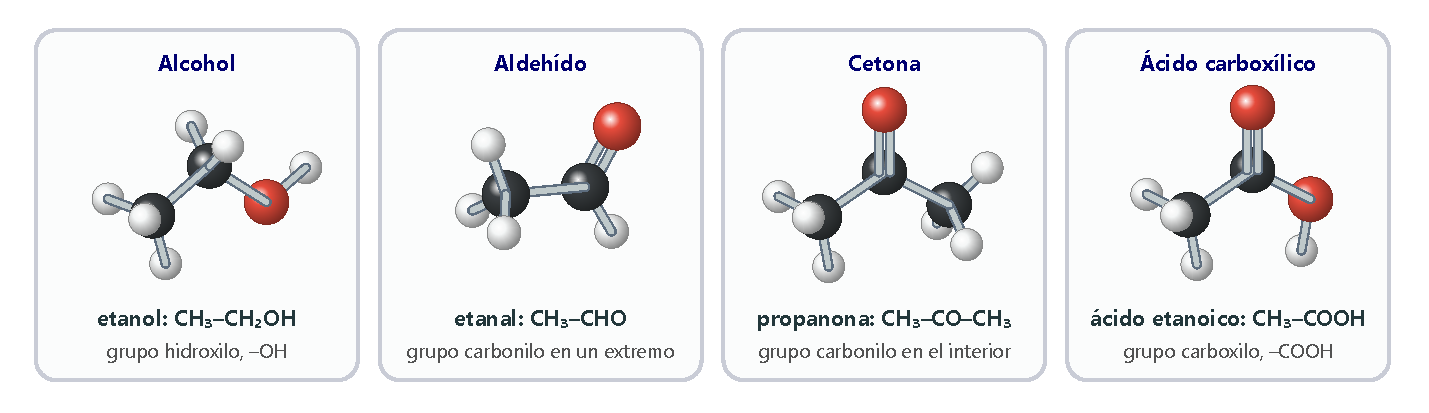
\includegraphics[width=\textwidth]{images/UD4/oxigenados}
    \caption{Modelos moleculares de algunos compuestos oxigenados.}
    \label{fig:oxigenados}
\end{figure}

\subsection{Los alcoholes}

Los \textbf{alcoholes} derivan de los hidrocarburos al sustituir uno o más hidrógenos por \textbf{grupos hidroxilo}, \ch{-OH}, que es su grupo funcional. Se nombran con el prefijo de la cadena principal, el localizador del grupo \ch{-OH} y la terminación \textbf{-ol}:

\begin{center}
    % --- tabla antigua ---
    % \begin{tblr}{colspec={lcl}, hlines, vlines, row{1}={bg=ocre!85, fg=white, font=\bfseries}, cells={font=\small}}
        % Semidesarrollada & Molecular & Nombre \\
        % \ch{CH3OH} & \ch{CH4O} & metanol \\
        % \ch{CH3-CH2OH} & \ch{C2H6O} & etanol \\
        % \ch{CH2OH-CH2-CH3} & \ch{C3H8O} & propan-1-ol \\
        % \ch{CH3-CHOH-CH3} & \ch{C3H8O} & propan-2-ol \\
        % \ch{CH2OH-CH2-CH2-CH3} & \ch{C4H10O} & butan-1-ol \\
    % \end{tblr}
    % --- tabla nueva ---
    {\small
    \begin{tabular}{@{}lcl@{}}
        \toprule
        \textbf{Semidesarrollada} & \textbf{Molecular} & \textbf{Nombre} \\
        \midrule
        \ch{CH3OH} & \ch{CH4O} & metanol \\[3pt]
        \ch{CH3-CH2OH} & \ch{C2H6O} & etanol \\[3pt]
        \ch{CH2OH-CH2-CH3} & \ch{C3H8O} & propan-1-ol \\[3pt]
        \ch{CH3-CHOH-CH3} & \ch{C3H8O} & propan-2-ol \\[3pt]
        \ch{CH2OH-CH2-CH2-CH3} & \ch{C4H10O} & butan-1-ol \\
        \bottomrule
    \end{tabular}
    }
\end{center}

Según el carbono al que esté unido el grupo \ch{-OH}, un alcohol es \textbf{primario} (el carbono está unido a otro carbono), \textbf{secundario} (unido a dos carbonos) o \textbf{terciario} (unido a tres carbonos):
\[ \underset{\text{propan-1-ol (primario)}}{\ch{CH3-CH2-CH2OH}} \qquad \underset{\text{butan-2-ol (secundario)}}{\ch{CH3-CH2-CHOH-CH3}} \qquad \underset{\text{2-metilpropan-2-ol (terciario)}}{\chemfig{CH_3-C(-[2]CH_3)(-[6]CH_3)-OH}} \]

\paragraph{Propiedades.} Los alcoholes tienen puntos de fusión y de ebullición más altos que los hidrocarburos con el mismo número de carbonos. El enlace O--H está polarizado: el hidrógeno tiene una carga parcial positiva (\(\delta+\)) y el oxígeno una negativa (\(\delta-\)), lo que permite que se formen \textbf{enlaces de hidrógeno} entre las moléculas (figura~\ref{fig:enlace_hidrogeno_alcoholes}). Los primeros alcoholes son solubles en agua en cualquier proporción, pero la solubilidad disminuye al crecer la cadena; también se disuelven en disolventes apolares.

\begin{center}
    % --- tabla antigua ---
    % \begin{tblr}{colspec={lc}, hlines, vlines, row{1}={bg=ocre!85, fg=white, font=\bfseries}, cells={font=\small}}
        % Compuesto & \(T_\text{eb}\) (\unit{\degreeCelsius}) \\
        % Metanol & \num{64.5} \\
        % Etanol & \num{78.0} \\
        % Propan-1-ol & \num{97.8} \\
        % Propan-2-ol & \num{82.3} \\
        % Butan-1-ol & \num{117.0} \\
    % \end{tblr}
    % --- tabla nueva ---
    {\small
    \begin{tabular}{@{}lc@{}}
        \toprule
        \textbf{Compuesto} & \textbf{\(T_\text{eb}\) (\unit{\degreeCelsius})} \\
        \midrule
        Metanol & \num{64.5} \\[3pt]
        Etanol & \num{78.0} \\[3pt]
        Propan-1-ol & \num{97.8} \\[3pt]
        Propan-2-ol & \num{82.3} \\[3pt]
        Butan-1-ol & \num{117.0} \\
        \bottomrule
    \end{tabular}
    }
    \qquad
    % --- tabla antigua ---
    % \begin{tblr}{colspec={lc}, hlines, vlines, row{1}={bg=ocre!85, fg=white, font=\bfseries}, cells={font=\small}}
        % Compuesto & \(T_\text{eb}\) (\unit{\degreeCelsius}) \\
        % Propano & \num{-42} \\
        % Butano & \num{-0.5} \\
        % Propanal & \num{49} \\
        % Propanona & \num{56} \\
        % Ácido propanoico & \num{141} \\
    % \end{tblr}
    % --- tabla nueva ---
    {\small
    \begin{tabular}{@{}lc@{}}
        \toprule
        \textbf{Compuesto} & \textbf{\(T_\text{eb}\) (\unit{\degreeCelsius})} \\
        \midrule
        Propano & \num{-42} \\[3pt]
        Butano & \num{-0.5} \\[3pt]
        Propanal & \num{49} \\[3pt]
        Propanona & \num{56} \\[3pt]
        Ácido propanoico & \num{141} \\
        \bottomrule
    \end{tabular}
    }
\end{center}

\begin{figure}[H]
    \centering
    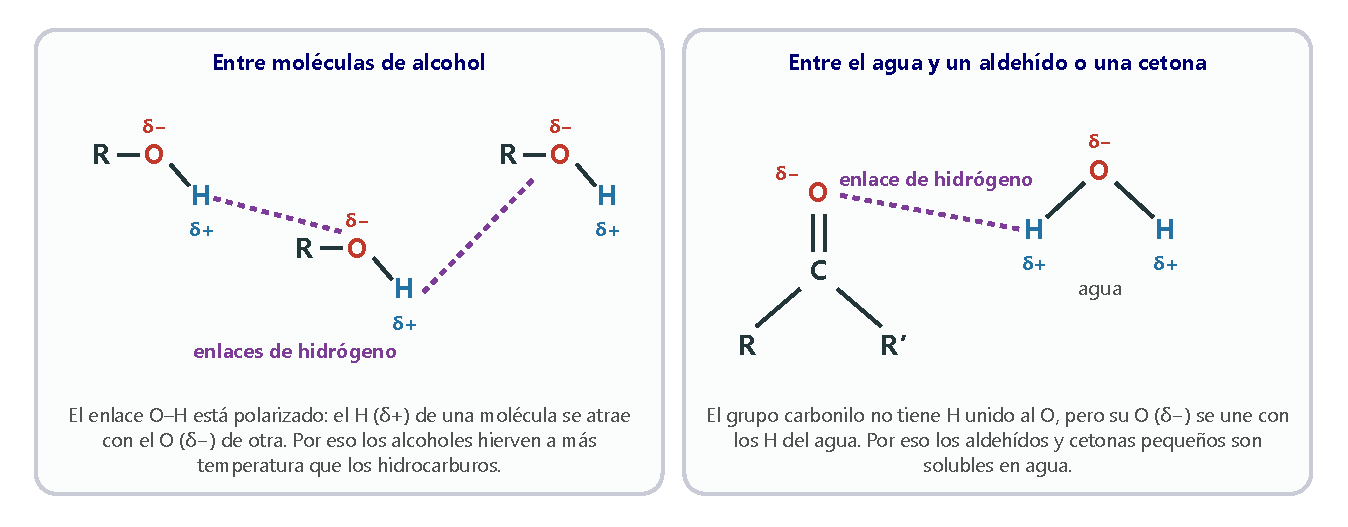
\includegraphics[width=\textwidth]{images/UD4/enlace_hidrogeno}
    \caption{Enlaces de hidrógeno entre moléculas de alcohol y entre el agua y un grupo carbonilo.}
    \label{fig:enlace_hidrogeno_alcoholes}
\end{figure}

\subsection{Los aldehídos y las cetonas}

Los \textbf{aldehídos} y las \textbf{cetonas} tienen el \textbf{grupo carbonilo}, C=O. En los aldehídos está en un \textbf{extremo} de la cadena (\ch{R-CHO}), y en las cetonas, en el \textbf{interior} (\ch{R-CO-R'}).

\paragraph{Nomenclatura.} Los \textbf{aldehídos} se nombran cambiando la -o final del hidrocarburo por \textbf{-al}. La cadena se numera siempre desde el carbono del grupo \ch{-CHO}, así que no hace falta indicar su posición; si hay dos grupos aldehído, se usa \textbf{-dial}. Por ejemplo, \ch{CH3-CH2-CH2-CHO} es el \textbf{butanal} y \ch{CHO-CH2-CH2-CHO}, el \textbf{butanodial}.

Las \textbf{cetonas} se nombran con la terminación \textbf{-ona}, indicando la posición del grupo carbonilo con el localizador más bajo posible: \ch{CH3-CO-CH2-CH3} es la \textbf{butanona}; \ch{CH3-CO-CH2-CH2-CH3}, la \textbf{pentan-2-ona}, y \ch{CH3-CH2-CO-CH2-CH3}, la \textbf{pentan-3-ona}. La cetona más sencilla es la propanona, o \textbf{acetona}, que se usa como disolvente (por ejemplo, en los quitaesmaltes).

\paragraph{Propiedades.} El grupo carbonilo es polar, por lo que los aldehídos y las cetonas hierven a más temperatura que los compuestos apolares de masa parecida. Sin embargo, como no tienen hidrógenos unidos al oxígeno, \textbf{no forman enlaces de hidrógeno entre sus moléculas}, y por eso hierven a menos temperatura que los alcoholes con el mismo número de carbonos. Sí pueden formar enlaces de hidrógeno con el agua (figura~\ref{fig:enlace_hidrogeno_alcoholes}), así que los que tienen pocos carbonos son solubles en agua; también se disuelven en disolventes apolares.

\subsection{Los ácidos carboxílicos y los ésteres}

Los \textbf{ácidos carboxílicos} tienen el \textbf{grupo carboxilo}, \ch{-COOH}, que siempre está en un extremo de la cadena (o en los dos). Se nombran con la palabra \emph{ácido} y la terminación \textbf{-oico}: \ch{HCOOH}, ácido metanoico (fórmico, el de las picaduras de hormiga); \ch{CH3-COOH}, ácido etanoico (acético, el del vinagre); \ch{CH3-CH2-COOH}, ácido propanoico; \ch{CH3-CH2-CH2-COOH}, ácido butanoico.

Los que tienen pocos carbonos son líquidos, y los de más de ocho carbonos son sólidos. Sus puntos de fusión y de ebullición aumentan con el número de carbonos y son los más altos de los compuestos oxigenados, porque forman enlaces de hidrógeno muy fuertes.

Al reaccionar un ácido carboxílico con un alcohol se forma un \textbf{éster} y agua. Los ésteres, con el grupo \ch{-COO\bond{single}}, son responsables del olor y el sabor de muchas frutas y se usan como aromas; por ejemplo, el etanoato de metilo, \ch{CH3-COO-CH3}.

\begin{exercise}
    El etanol es el alcohol más conocido. Busca información sobre sus aplicaciones.
    \begin{solu}
        Respuesta libre. Se usa como \textcolor{red}{desinfectante} (en los geles hidroalcohólicos), como \textcolor{red}{disolvente} (perfumes, medicamentos), como \textcolor{red}{biocombustible} mezclado con la gasolina y está presente en las \textcolor{red}{bebidas alcohólicas}.
    \end{solu}
\end{exercise}

\begin{exercise}
    Formula estos alcoholes y clasifícalos en primarios, secundarios o terciarios: a) butan-1-ol; b) butan-2-ol; c) 2-metilbutan-2-ol.
    \begin{solu}
        a) \ch{CH2OH-CH2-CH2-CH3}, \textcolor{red}{primario}. b) \ch{CH3-CHOH-CH2-CH3}, \textcolor{red}{secundario}.
        c) \[ \chemfig{CH_3-C(-[2]OH)(-[6]CH_3)-CH_2-CH_3} \] \textcolor{red}{terciario}.
    \end{solu}
\end{exercise}

\begin{exercise}
    ¿Cuál es el aldehído más sencillo? ¿Y la cetona más sencilla? Calcula su masa molecular.
    \begin{solu}
        El \textcolor{red}{metanal}, \ch{HCHO} (\ch{CH2O}): \(M = 12 + 2 + 16 = \textcolor{red}{30}\). La \textcolor{red}{propanona}, \ch{CH3-CO-CH3} (\ch{C3H6O}): \(M = 36 + 6 + 16 = \textcolor{red}{58}\).
    \end{solu}
\end{exercise}

\subsection*{Actividades de consolidación: los compuestos oxigenados}

\begin{exercise}
    Vertemos \qty{5}{\mL} de etanol en tres tubos de ensayo. a) Observa el primero: ¿en qué estado está el etanol? ¿Cómo son su color y su olor? b) Al segundo le añadimos agua: ¿es soluble el etanol en agua? c) Al tercero le añadimos un disolvente apolar: ¿es soluble en él?
    \begin{solu}
        a) Es un \textcolor{red}{líquido incoloro} con un \textcolor{red}{olor característico}. b) Es \textcolor{red}{muy soluble} en agua (por su grupo \ch{-OH}). c) También es \textcolor{red}{soluble} en disolventes apolares (por su parte \ch{CH3-CH2\bond{single}}).
    \end{solu}
\end{exercise}

\begin{exercise}
    Formula: a) metanol; b) propan-2-ol; c) butan-1-ol; d) pentan-2-ol.
    \begin{solu}
        a) \textcolor{red}{\ch{CH3OH}}; b) \textcolor{red}{\ch{CH3-CHOH-CH3}};
        c) \textcolor{red}{\ch{CH2OH-CH2-CH2-CH3}}; d) \textcolor{red}{\ch{CH3-CHOH-CH2-CH2-CH3}}.
    \end{solu}
\end{exercise}

\begin{exercise}
    Clasifica estos alcoholes en primarios, secundarios o terciarios:
    \[ \text{a)}\ \chemfig{CH_3-C(-[2]OH)(-[6]CH_3)-CH_2-CH_3} \qquad \text{b)}\ \ch{CH3-CH2OH} \]
    \[ \text{c)}\ \chemfig{CH_3-C(-[2]OH)(-[6]CH_3)-CH_3} \qquad \text{d)}\ \ch{CH3OH} \]
    \begin{solu}
        b) y d) son \textcolor{red}{primarios} (el metanol se considera primario). a) y c) son \textcolor{red}{terciarios}.
    \end{solu}
\end{exercise}

\begin{exercise}
    Indica si son primarios, secundarios o terciarios y escribe su fórmula desarrollada: A: \ch{CH2OH-CH2-CH3}; B: \ch{CH3-CHOH-CH3}.
    \begin{solu}
        A: propan-1-ol, \textcolor{red}{primario}: \[ \chemfig{H-C(-[2]H)(-[6]H)-C(-[2]H)(-[6]H)-C(-[2]H)(-[6]H)-O-H} \]

        B: propan-2-ol, \textcolor{red}{secundario}: \[ \chemfig{H-C(-[2]H)(-[6]H)-C(-[2]OH)(-[6]H)-C(-[2]H)(-[6]H)-H} \]
    \end{solu}
\end{exercise}

\begin{exercise}
    ¿Por qué los alcoholes hierven a mayor temperatura que los hidrocarburos con el mismo número de carbonos? ¿Por qué los primeros alcoholes son solubles en agua?
    \begin{solu}
        Porque el enlace O--H está \textcolor{red}{polarizado} y entre las moléculas de alcohol se forman \textcolor{red}{enlaces de hidrógeno}, que hay que romper para que el líquido hierva. Por la misma razón, el grupo \ch{-OH} forma enlaces de hidrógeno con el agua: los alcoholes de \textcolor{red}{cadena corta} se disuelven en agua en cualquier proporción; al crecer la cadena (parte apolar), la solubilidad disminuye.
    \end{solu}
\end{exercise}

\begin{exercise}
    Formula: a) butanal; b) 2-metilbutanal; c) hexan-3-ona; d) 2-metilpentan-3-ona; e) ácido 3-metilbutanoico; f) ácido 4-metilpentanoico.
    \begin{solu}
        \[ \text{a)}\ \textcolor{red}{\ch{CH3-CH2-CH2-CHO}} \]
        \[ \text{b)}\ \textcolor{red}{\chemfig{CH_3-CH_2-CH(-[6]CH_3)-CHO}} \]
        \[ \text{c)}\ \textcolor{red}{\ch{CH3-CH2-CO-CH2-CH2-CH3}} \]

        \[ \text{d)}\ \textcolor{red}{\chemfig{CH_3-CH(-[6]CH_3)-CO-CH_2-CH_3}} \]
        \[ \text{e)}\ \textcolor{red}{\chemfig{CH_3-CH(-[6]CH_3)-CH_2-COOH}} \]

        \[ \text{f)}\ \textcolor{red}{\chemfig{CH_3-CH(-[6]CH_3)-CH_2-CH_2-COOH}} \]
    \end{solu}
\end{exercise}

\begin{exercise}
    Nombra: a) \ch{CH3-CH2-CH2-COOH}; b) \ch{CH3-CH2-CH2-CH2-CH2-CHO}.
    \begin{solu}
        a) \textcolor{red}{Ácido butanoico}. b) \textcolor{red}{Hexanal}.
    \end{solu}
\end{exercise}

\begin{exercise}
    Señala si es verdadero o falso: a) El butan-2-ol es un alcohol primario. b) El grupo funcional de los aldehídos es \ch{-CHO}. c) Los alcoholes son insolubles en agua. d) El ácido etanoico está en el vinagre.
    \begin{solu}
        a) \textcolor{red}{Falso}: es secundario. b) \textcolor{red}{Verdadero}. c) \textcolor{red}{Falso}: los de cadena corta son muy solubles. d) \textcolor{red}{Verdadero}.
    \end{solu}
\end{exercise}

\begin{exercise}
    Formula: a) etanol; b) ácido etanoico; c) etanal.
    \begin{solu}
        a) \textcolor{red}{\ch{CH3-CH2OH}}; b) \textcolor{red}{\ch{CH3-COOH}}; c) \textcolor{red}{\ch{CH3-CHO}}.
    \end{solu}
\end{exercise}

\begin{exercise}
    Indica si es verdadero o falso y justifica tu respuesta:
    \begin{enumerate}[label=\alph*)]
        \item Los aldehídos y las cetonas hierven a más temperatura que los alcoholes con igual número de carbonos.
        \item Un aldehído o una cetona pueden ser solubles en disolventes polares y apolares.
        \item El grupo carbonilo es el grupo funcional de los ácidos carboxílicos.
        \item El grupo carboxilo es el grupo funcional de las cetonas.
        \item El ácido butanoico hierve a más temperatura que el ácido metanoico.
    \end{enumerate}
    \begin{solu}
        a) \textcolor{red}{Falso}: hierven a menos temperatura, porque no forman enlaces de hidrógeno entre sus moléculas. b) \textcolor{red}{Verdadero}. c) \textcolor{red}{Falso}: es el grupo carboxilo, \ch{-COOH}. d) \textcolor{red}{Falso}: es el grupo carbonilo, C=O. e) \textcolor{red}{Verdadero}: tiene más carbonos.
    \end{solu}
\end{exercise}

%========================================================================================
\section[Las aminas]{¿Qué son los compuestos nitrogenados? Las aminas}
%========================================================================================

Las \textbf{aminas} son compuestos en los que uno, dos o los tres hidrógenos del amoníaco, \ch{NH3}, se sustituyen por cadenas carbonadas. Su grupo funcional es el \textbf{grupo amino}, \ch{-NH2} (figura~\ref{fig:aminas}):
\begin{itemize}
    \item \textbf{Aminas primarias}, \ch{R-NH2}: se sustituye un hidrógeno. Ejemplo: etilamina, \ch{CH3-CH2-NH2}.
    \item \textbf{Aminas secundarias}, \ch{R-NH-R'}: se sustituyen dos hidrógenos. Ejemplo: N-metiletilamina, \ch{CH3-CH2-NH-CH3}.
    \item \textbf{Aminas terciarias}, \ch{RR'R''N}: se sustituyen los tres. Ejemplo: trimetilamina, \ch{N(CH3)3}.
\end{itemize}

\begin{figure}[H]
    \centering
    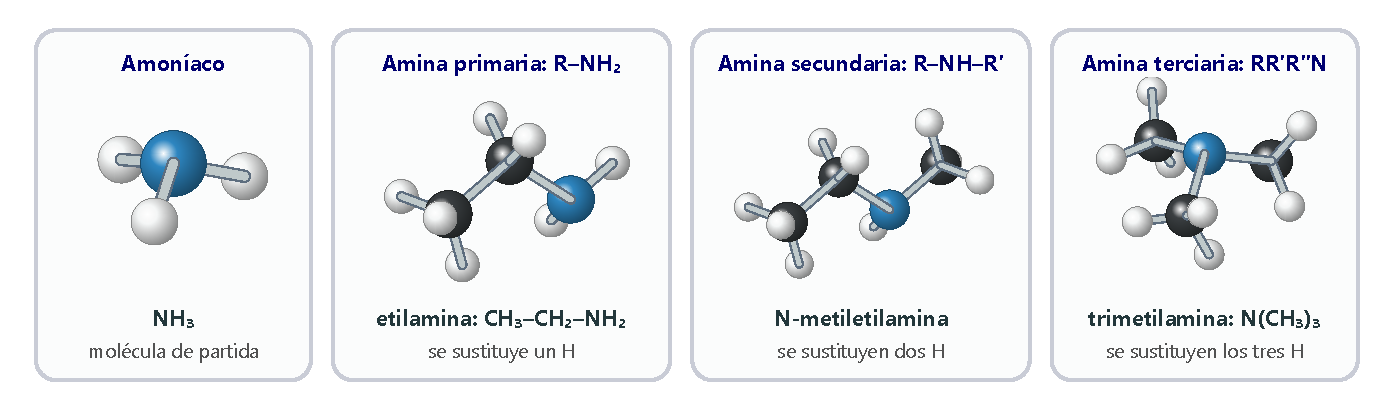
\includegraphics[width=\textwidth]{images/UD4/aminas}
    \caption{Modelos moleculares del amoníaco y de aminas primaria, secundaria y terciaria.}
    \label{fig:aminas}
\end{figure}

\paragraph{Nomenclatura.} Las aminas primarias se nombran añadiendo \textbf{-amina} al nombre del radical: \ch{CH3NH2}, metilamina. En las secundarias y terciarias, se pone \emph{-amina} detrás del radical más largo, y los demás radicales se nombran delante, en orden alfabético y precedidos de \emph{N-} para indicar que están unidos al nitrógeno: \ch{CH3-CH2-CH2-NH-CH3}, N-metilpropilamina; \ch{CH3-CH2-N(CH3)2}, N,N-dimetiletilamina.

\paragraph{Propiedades.} Las aminas primarias y secundarias tienen hidrógenos unidos al nitrógeno y forman enlaces de hidrógeno entre sus moléculas, aunque más débiles que los de los alcoholes. Por eso sus puntos de fusión y de ebullición están entre los de los hidrocarburos y los de los alcoholes de masa parecida. Las aminas de pocos carbonos son muy solubles en agua. Muchas tienen un olor desagradable (a pescado podrido, como la trimetilamina), y forman parte de los aminoácidos y de muchos medicamentos.

\subsection*{Actividades de consolidación: las aminas}

\begin{exercise}
    En la figura~\ref{fig:aminas}, ¿cuántos átomos de carbono están unidos al nitrógeno en cada amina? Relaciónalo con su clasificación.
    \begin{solu}
        En la etilamina, \textcolor{red}{uno} (primaria); en la N-metiletilamina, \textcolor{red}{dos} (secundaria); en la trimetilamina, \textcolor{red}{tres} (terciaria).
    \end{solu}
\end{exercise}

\begin{exercise}
    Formula estas aminas y clasifícalas: a) butilamina; b) N-metilpropilamina; c) N,N-dimetiletilamina; d) N-propilbutilamina.
    \begin{solu}
        a) \ch{CH3-CH2-CH2-CH2-NH2}, \textcolor{red}{primaria}. b) \ch{CH3-CH2-CH2-NH-CH3}, \textcolor{red}{secundaria}. c) \ch{CH3-CH2-N(CH3)2}, \textcolor{red}{terciaria}. d) \ch{CH3-CH2-CH2-CH2-NH-CH2-CH2-CH3}, \textcolor{red}{secundaria}.
    \end{solu}
\end{exercise}

\begin{exercise}
    Nombra la amina \ch{N(CH3)3} y calcula su masa molecular. ¿Es primaria, secundaria o terciaria?
    \begin{solu}
        Es la \textcolor{red}{trimetilamina}, \ch{C3H9N}: \(M = 36 + 9 + 14 = \textcolor{red}{59}\). Es \textcolor{red}{terciaria}.
    \end{solu}
\end{exercise}

\begin{exercise}
    Responde verdadero o falso y justifica tu respuesta: a) En las aminas secundarias se sustituyen dos hidrógenos del amoníaco por dos radicales. b) Las aminas primarias hierven a más temperatura que los hidrocarburos de masa parecida.
    \begin{solu}
        a) \textcolor{red}{Verdadero}. b) \textcolor{red}{Verdadero}: forman \textcolor{red}{enlaces de hidrógeno} entre sus moléculas gracias a los enlaces N--H, que están polarizados.
    \end{solu}
\end{exercise}

%========================================================================================
\section[Compuestos del carbono de especial interés]{¿Qué compuestos del carbono son de especial interés?}
%========================================================================================

Muchos compuestos del carbono tienen interés biológico, industrial o de ambos tipos.

\subsection{Los glúcidos y los lípidos}

Los \textbf{glúcidos} (hidratos de carbono) están formados por carbono, hidrógeno y oxígeno, y los fabrican las plantas verdes mediante la \textbf{fotosíntesis}. Son la principal fuente de energía de los seres vivos: la combustión de cada gramo de glúcidos proporciona al organismo unos \qty{17}{\kilo\joule}. La glucosa y la fructosa están en las frutas y son solubles en agua; la sacarosa (el azúcar común) está formada por una molécula de glucosa y otra de fructosa unidas.

Los \textbf{lípidos} también están formados por carbono, hidrógeno y oxígeno, pero no se disuelven en agua, sino en disolventes apolares. Los más comunes son las grasas, que almacenan más energía por unidad de masa que ningún otro alimento (unos \qty{37}{\kilo\joule\per\gram}). Son ricos en lípidos los aceites, la mantequilla, la nata o la manteca.

\subsection{Los polímeros}

Los \textbf{polímeros} están formados por macromoléculas que resultan de la unión de muchas moléculas pequeñas, los \textbf{monómeros}, en un proceso llamado \textbf{polimerización} (figura~\ref{fig:polietileno}).

\begin{figure}[H]
    \centering
    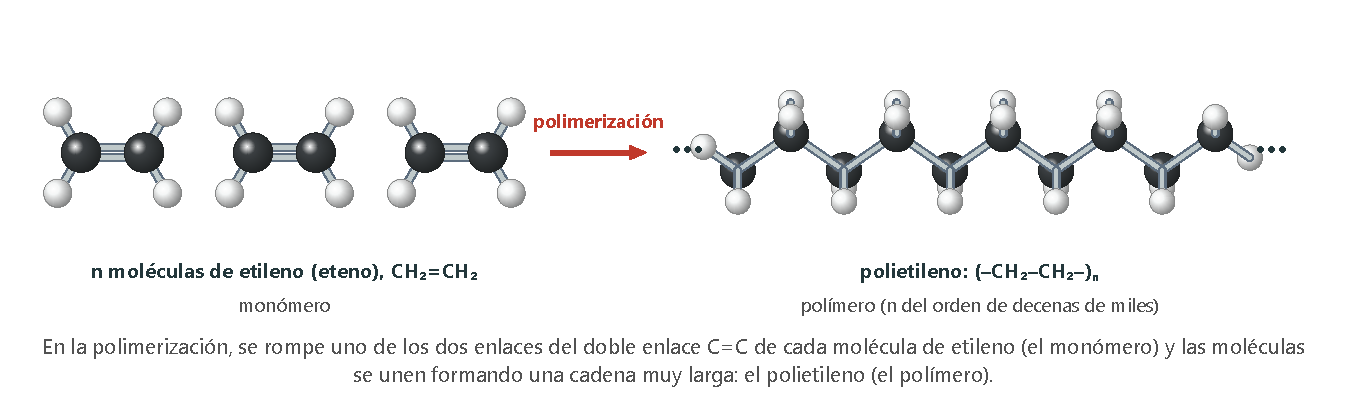
\includegraphics[width=\textwidth]{images/UD4/polietileno}
    \caption{El polietileno se forma por la unión de muchas moléculas de etileno.}
    \label{fig:polietileno}
\end{figure}

\begin{itemize}
    \item \textbf{Polímeros naturales}: el almidón, el glucógeno, la celulosa, las proteínas, los ácidos nucleicos o el caucho. La \textbf{celulosa} es el compuesto del carbono más abundante en la naturaleza; está formada por cadenas de cientos o miles de moléculas de glucosa y es la materia prima del papel y de fibras como el algodón o el lino. El \textbf{caucho} es un polímero del isopreno que se extrae del látex de algunas plantas; se vulcaniza (se calienta con azufre) para que sea más resistente.
    \item \textbf{Polímeros artificiales}: gran parte de la industria química se dedica a fabricar plásticos y fibras artificiales. Se clasifican en:
    \begin{itemize}
        \item \textbf{Termoplásticos}: se reblandecen al calentarlos y recuperan la rigidez al enfriarse, por lo que se pueden moldear y reciclar. Ejemplos: polietileno, poliestireno, PVC, PET.
        \item \textbf{Termoestables}: una vez endurecidos, no se reblandecen al calentarlos. Ejemplos: baquelita, resinas de melamina y epoxi.
        \item \textbf{Elastómeros}: muy elásticos y blandos, formados por cadenas muy largas plegadas sobre sí mismas. Ejemplos: el caucho artificial y el neopreno.
    \end{itemize}
\end{itemize}

\begin{exercise}
    Durante la Primera Guerra Mundial, el caucho natural escaseaba y era carísimo. Científicos estadounidenses y alemanes, de forma independiente, desarrollaron cauchos sintéticos, como el neopreno (1930). Busca información sobre el contexto económico y político de estas investigaciones.
    \begin{solu}
        Respuesta libre. El caucho natural procedía casi todo de plantaciones de Asia controladas por potencias coloniales, y durante las guerras su suministro se cortaba (el bloqueo naval afectó sobre todo a Alemania). Disponer de \textcolor{red}{caucho sintético} se consideraba estratégico para la industria y el ejército (neumáticos, juntas\ldots).
    \end{solu}
\end{exercise}

\subsection*{Actividades de consolidación: compuestos de especial interés}

\begin{exercise}
    ¿Qué son los glúcidos? ¿Qué función tienen en los seres vivos? Nombra algunos y di en qué alimentos se encuentran.
    \begin{solu}
        Son compuestos de \textcolor{red}{carbono, hidrógeno y oxígeno} que constituyen la \textcolor{red}{principal fuente de energía} de los seres vivos. Ejemplos: glucosa y fructosa (frutas, miel), sacarosa (azúcar), almidón (pan, pasta, patatas, arroz).
    \end{solu}
\end{exercise}

\begin{exercise}
    Relaciona cada característica con los glúcidos, los lípidos o ambos: a) solubles en agua; b) insolubles en agua; c) aceites y grasas; d) fuente de energía de los seres vivos; e) formados por C, H y O; f) se obtienen por fotosíntesis.
    \begin{solu}
        a) \textcolor{red}{Glúcidos} (los sencillos); b) \textcolor{red}{lípidos}; c) \textcolor{red}{lípidos}; d) \textcolor{red}{ambos}; e) \textcolor{red}{ambos}; f) \textcolor{red}{glúcidos}.
    \end{solu}
\end{exercise}

\begin{exercise}
    El polietileno tiene la cadena \((\ldots\ch{-CH2-CH2-CH2-CH2-CH2\bond{single}}\ldots)\), con unas \num{100000} unidades \ch{-CH2\bond{single}}. ¿Cuál es su monómero? Si cada molécula de etileno aporta dos unidades, ¿cuántas moléculas de etileno forman una cadena?
    \begin{solu}
        El monómero es el \textcolor{red}{etileno (eteno), \ch{CH2=CH2}}, \ch{C2H4}. Una cadena contiene unas \(\num{100000}/2 = \textcolor{red}{\num{50000}}\) moléculas de etileno.
    \end{solu}
\end{exercise}

\begin{exercise}
    Clasifica en naturales o artificiales: almidón, PVC, celulosa y neopreno.
    \begin{solu}
        Naturales: \textcolor{red}{almidón y celulosa}. Artificiales: \textcolor{red}{PVC y neopreno}.
    \end{solu}
\end{exercise}
